\documentclass[aspectratio=169,c]{beamer}
\usetheme{default}
\usecolortheme{dove}
\setbeamertemplate{navigation symbols}{}

% ── Fonts and microtypography ──────────────────────────────────
\usepackage{lmodern}
\usepackage{microtype}

% ── Color palette ──────────────────────────────────────────────
\definecolor{primary}{RGB}{23,63,95}
\definecolor{medgray}{RGB}{140,140,140}

\setbeamercolor{title}{fg=primary}
\setbeamercolor{subtitle}{fg=medgray}
\setbeamercolor{frametitle}{fg=primary}
\setbeamercolor{structure}{fg=primary}

% ── Frame titles (centered, colored) ──────────────────────────
\setbeamertemplate{frametitle}[default][center]

% ── Title page ─────────────────────────────────────────────────
\setbeamertemplate{title page}{
  \vfill
  \centering
  {\color{primary!40}\rule{0.45\textwidth}{0.4pt}}\\[1.5em]
  {\usebeamerfont{title}\usebeamercolor[fg]{title}\inserttitle}\\[0.8em]
  {\usebeamerfont{subtitle}\usebeamercolor[fg]{subtitle}\insertsubtitle}\\[1.5em]
  {\color{primary!40}\rule{0.45\textwidth}{0.4pt}}
  \vfill
}

% ── Footline ───────────────────────────────────────────────────
\newcommand{\defaultfootline}{%
  \setbeamertemplate{footline}{%
    \hfill{\color{medgray}\scriptsize\insertframenumber\kern14pt}\vskip6pt%
  }%
}
\defaultfootline

\newcommand{\hideframenumber}{%
  \setbeamertemplate{footline}{}%
  \addtocounter{framenumber}{-1}%
}
\newcommand{\showframenumber}{\defaultfootline}

% ── Section pages ────────────────────────────────────────────
\setbeamertemplate{section page}{
  \centering
  \vfill
  {\color{primary!40}\rule{0.35\textwidth}{0.4pt}}\\[1.2em]
  {\LARGE\bfseries\color{primary}\thesection.~\insertsection}\\[1.2em]
  {\color{primary!40}\rule{0.35\textwidth}{0.4pt}}
  \vfill
}

% ── Spacing ────────────────────────────────────────────────────
\setbeamertemplate{itemize/enumerate body begin}{\setlength\itemsep{6pt}}
\setbeamertemplate{itemize/enumerate subbody begin}{\setlength\itemsep{4pt}}
\renewcommand{\arraystretch}{1.25}

\setbeamertemplate{footline}[frame number]

% ==============================================================
\title{Compound vs Isolated Cyclone Shocks}
\subtitle{Do Repeated Shocks Compound the Damage?}

\begin{document}

{\hideframenumber
\begin{frame}
\titlepage
\end{frame}
\showframenumber}

% ===============================================================
\section{Motivation and Data}
% ===============================================================

{\hideframenumber
\begin{frame}
\sectionpage
\end{frame}
\showframenumber}

\begin{frame}{Question}
Do cyclone shocks that follow closely after a previous shock --- \textbf{compound shocks} --- cause more or less damage than \textbf{isolated shocks}?

\medskip
Two competing hypotheses:
\begin{itemize}
  \item \textbf{Compounding damage}: A second shock hits while the economy is still recovering, amplifying the GDP loss (weakened infrastructure, depleted reserves)
  \item \textbf{Diminishing marginal damage}: The first shock already destroyed vulnerable capital, so a second shock has less left to destroy; or governments pre-position response capacity after the first event
\end{itemize}

\medskip
\textbf{Definition}: A shock in year $t$ is \emph{compound} if there was also a p95 cyclone shock in $t{-}1$. Otherwise it is \emph{isolated}.
\end{frame}

\begin{frame}{The Threshold Problem}
The baseline p95 threshold is computed across \emph{all} country-years (88\% of which have zero wind speed), yielding a threshold of just \textbf{60 knots} --- barely tropical storm strength.

\medskip
This means large cyclone-prone countries are ``treated'' nearly every year:

\centering
\smallskip
\begin{tabular}{l r r r r}
\hline
\textbf{Country} & \textbf{p95 (60 kts)} & \textbf{Cat 1+ (64)} & \textbf{Cat 2+ (83)} & \textbf{Cat 3+ (96)} \\
\hline
Australia & 41 / 46 yrs & 40 & 25 & 14 \\
China     & 44 / 46 yrs & 41 & 13 & 7  \\
Philippines & 42 / 46 yrs & 39 & 30 & 17 \\
Japan     & 40 / 46 yrs & 37 & 11 & 4  \\
\hline
\end{tabular}

\smallskip
\small
\begin{itemize}
  \item At p95, these countries have $\geq 90\%$ compound shocks $\to$ no within-country variation
  \item Higher thresholds (Cat 2+, Cat 3+) capture only severe events and produce more isolated shocks
\end{itemize}
\end{frame}

\begin{frame}{Shock Classification (Baseline p95)}
\centering
\begin{tabular}{l r r}
\hline
& \textbf{Count} & \textbf{Share} \\
\hline
Total shock-years & 423 & 100\% \\
Compound (strict: shock in $t{-}1$) & 260 & 61.5\% \\
Isolated (no shock in $t{-}1$) & 163 & 38.5\% \\
\hline
Compound (broad: shock in $t{-}1$ or $t{-}2$) & 311 & 73.5\% \\
Isolated (broad: no shock in $t{-}1$ or $t{-}2$) & 112 & 26.5\% \\
\hline
\end{tabular}

\bigskip
\begin{itemize}
  \item Among the 40 ever-treated countries, nearly two-thirds of all shock-years are compound
  \item Compound share is stable across periods: 62.6\% pre-1990, 60.6\% post-1990
  \item 19 countries have \emph{both} compound and isolated shocks $\to$ within-country variation exists
\end{itemize}
\end{frame}

\begin{frame}{Shock Composition Across Thresholds}
\centering
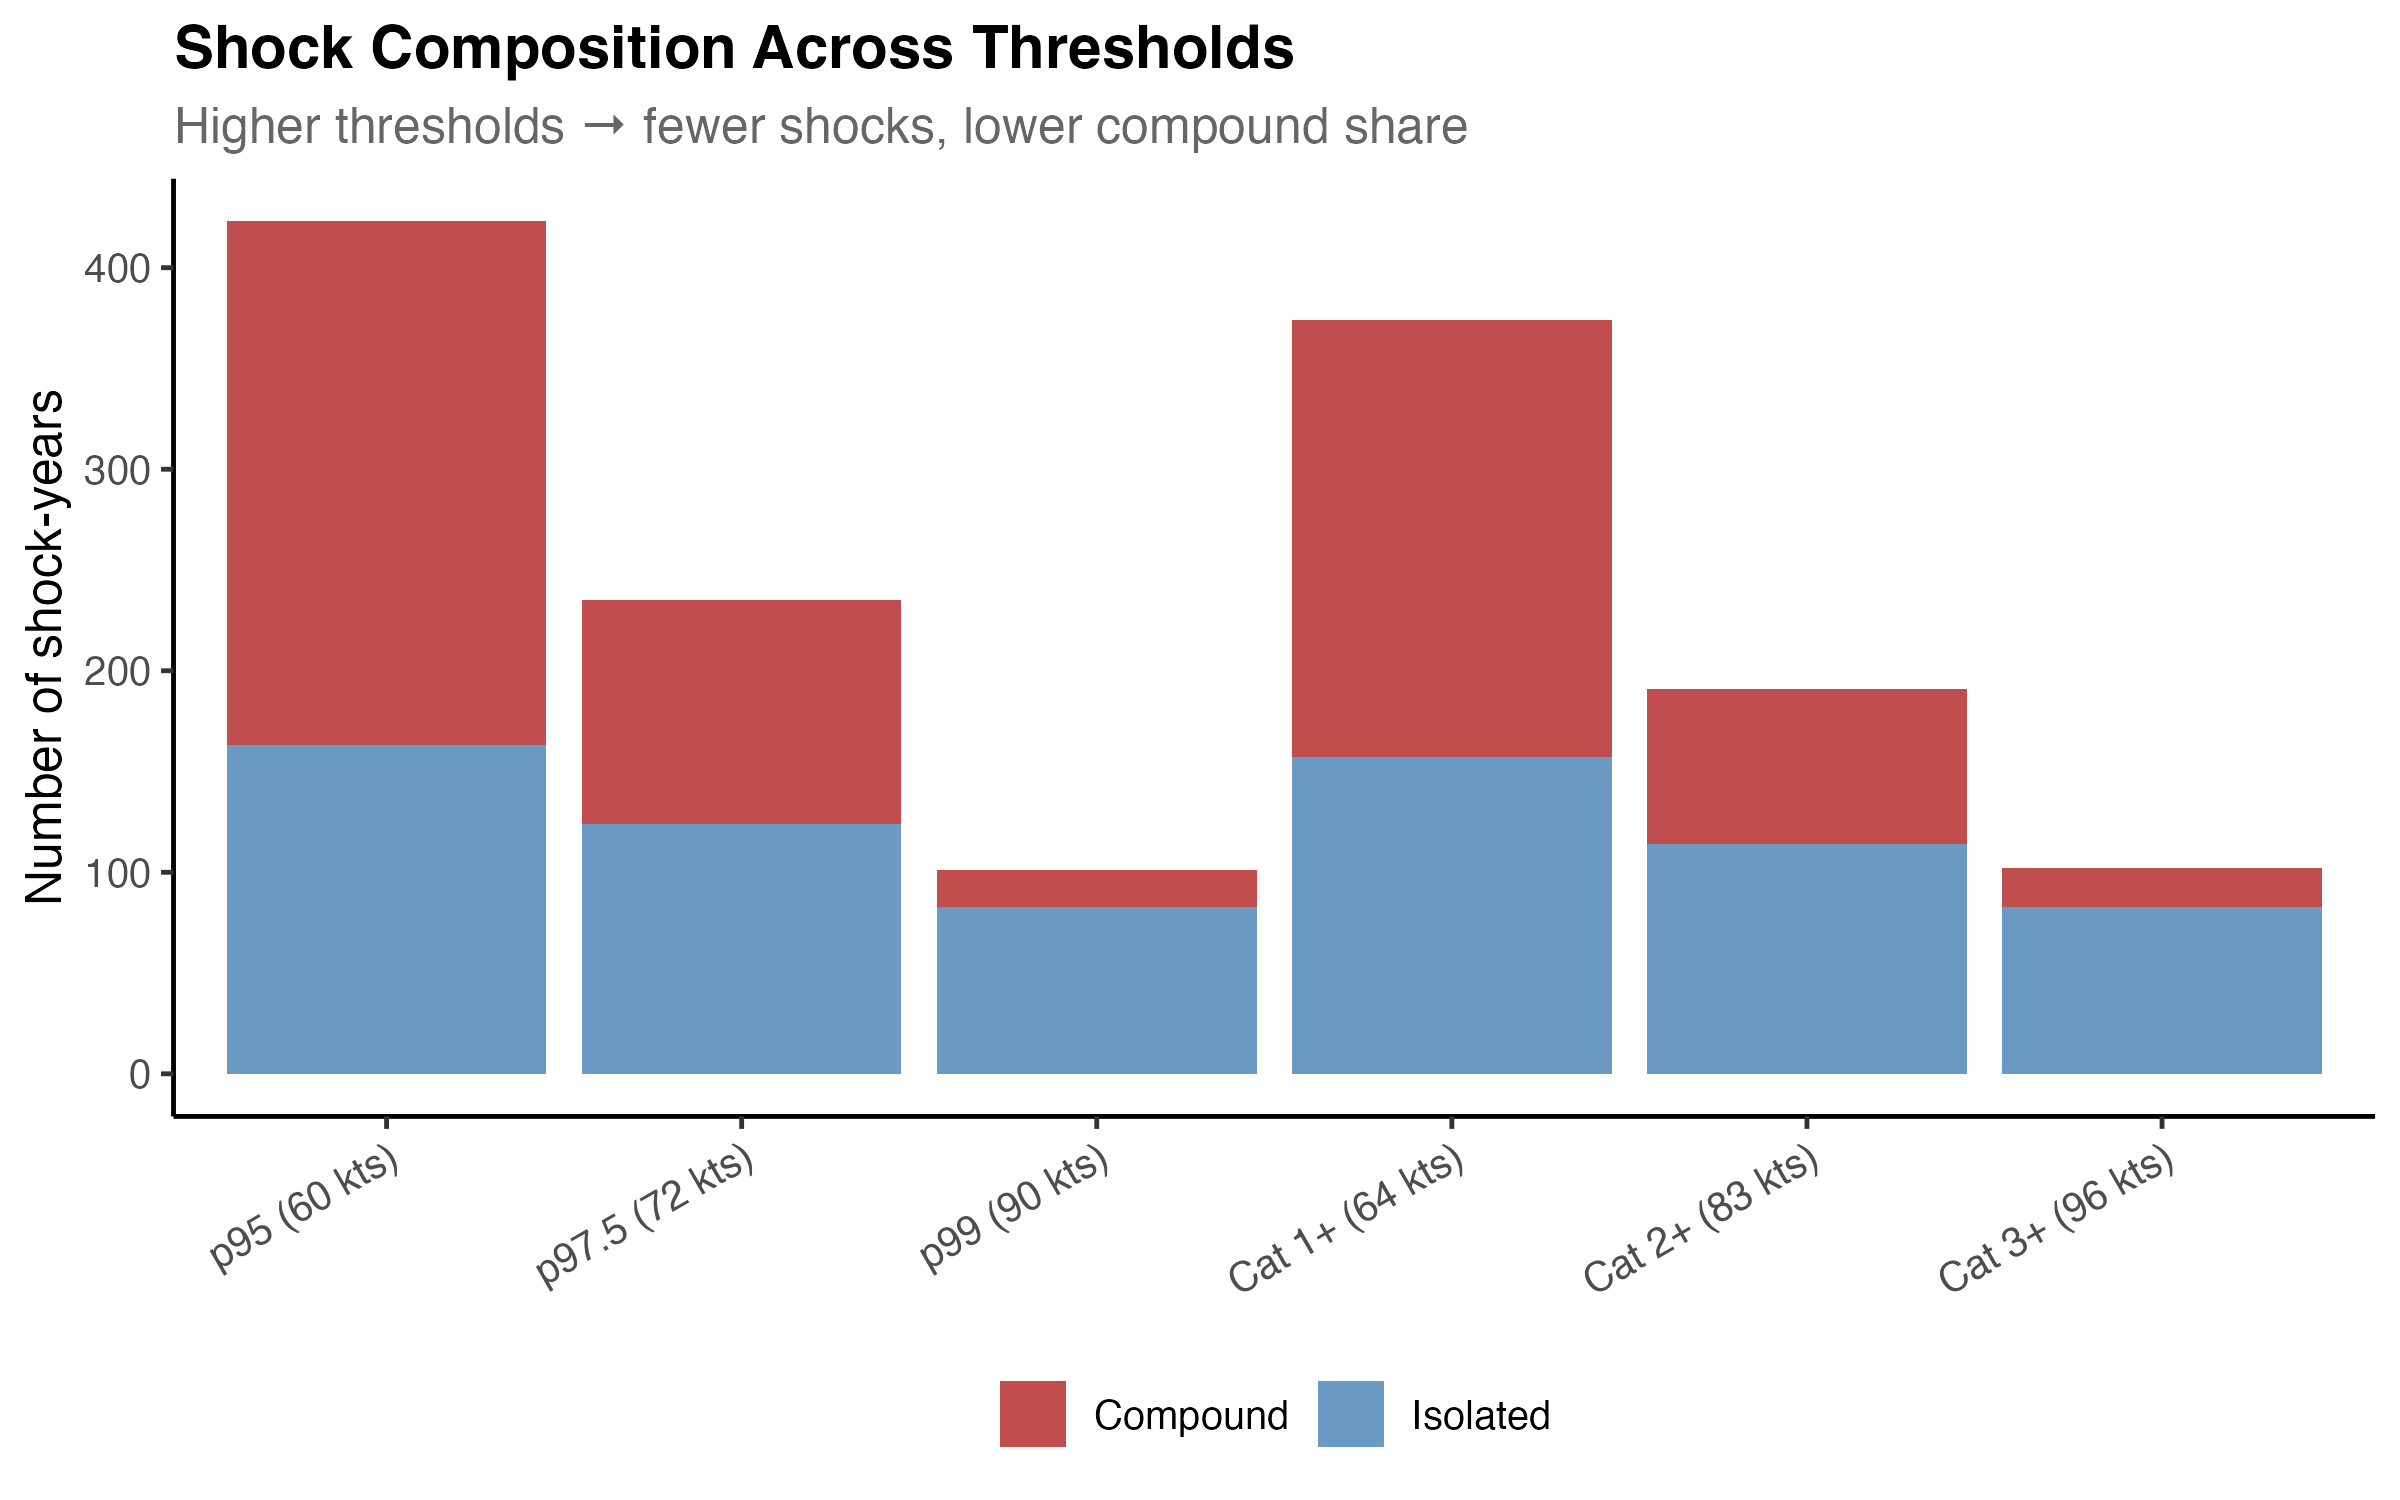
\includegraphics[width=0.72\textwidth,height=0.60\textheight,keepaspectratio]{figures/threshold_composition.png}

\smallskip
\small
Higher thresholds sharply reduce both total shocks and the compound share: from 61.5\% (p95) to 18\% (Cat 3+). At Cat 2+ (83 knots), there are 191 shocks with a 40\% compound share --- a reasonable balance of power and variation.
\end{frame}

\begin{frame}{Shock Timeline: Selected Countries}
\centering
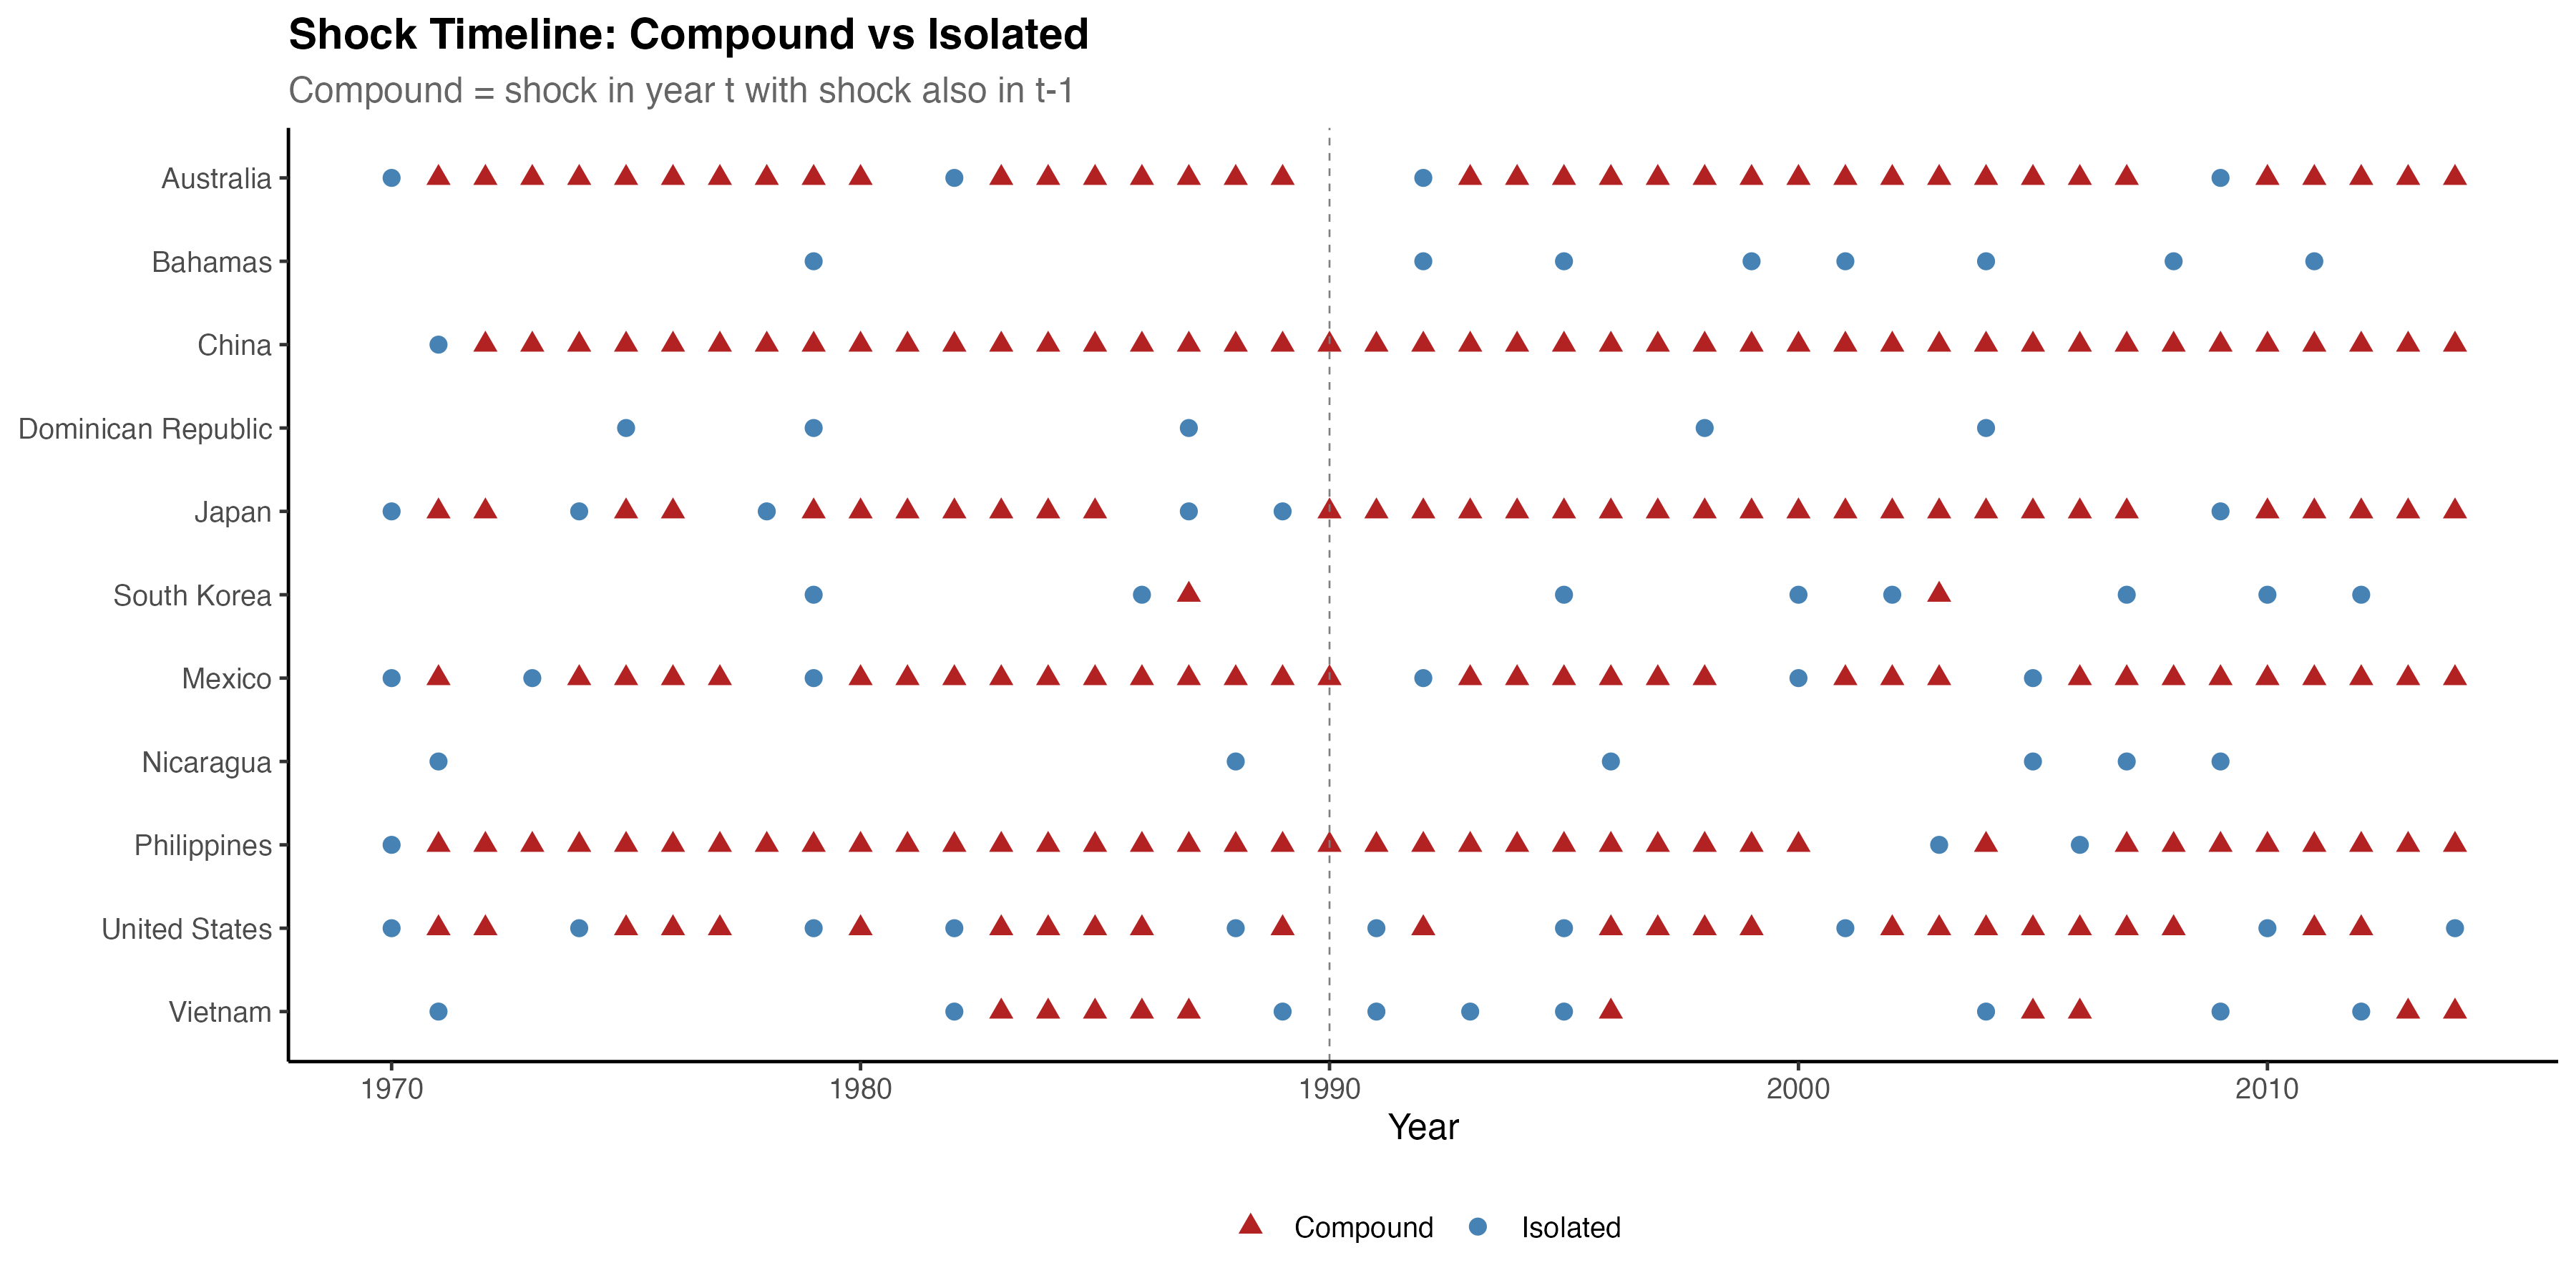
\includegraphics[width=\textwidth,height=0.72\textheight,keepaspectratio]{figures/shock_timeline.png}

\smallskip
\small
Large cyclone-prone countries (CHN, PHL, AUS, JPN, MEX) are hit nearly every year $\to$ almost all compound. Smaller Caribbean countries (BHS, NIC, DOM) have sporadic, isolated shocks.
\end{frame}

\begin{frame}{Inter-Shock Gap Distribution}
\centering
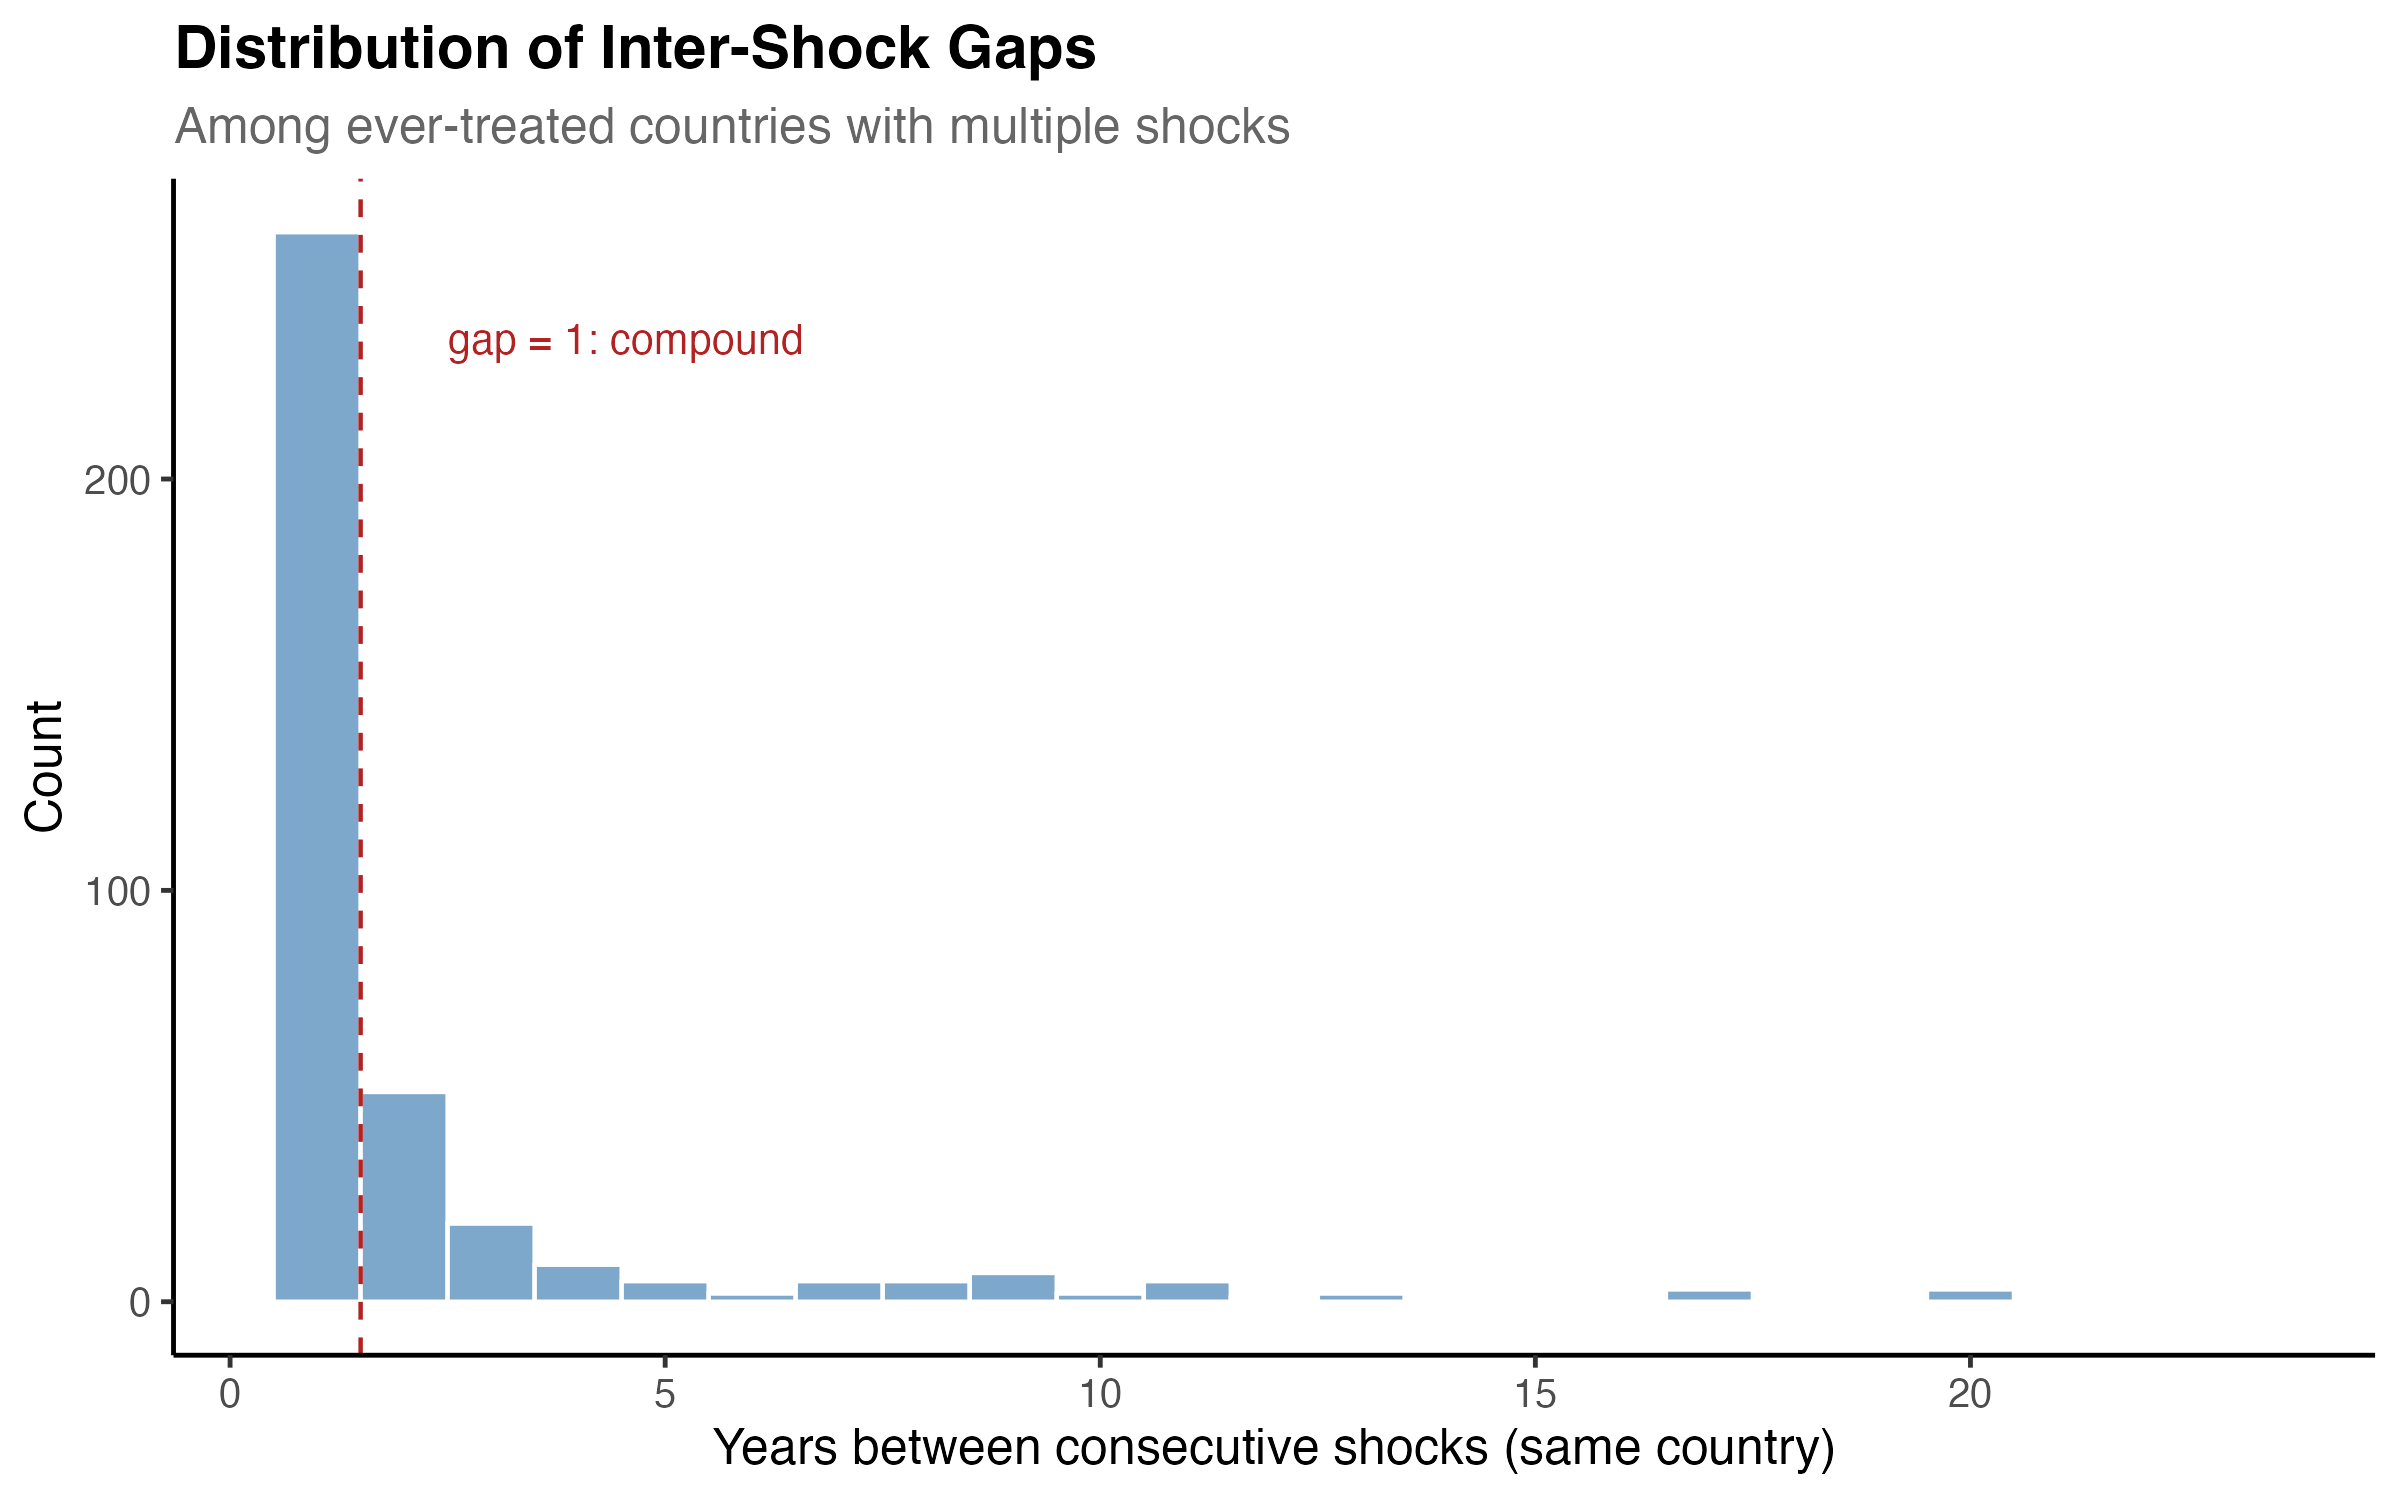
\includegraphics[width=0.72\textwidth,height=0.62\textheight,keepaspectratio]{figures/gap_distribution.png}

\smallskip
\small
The modal gap between consecutive shocks within a country is \textbf{1 year}. Most multi-shock countries experience near-continuous exposure, not discrete, well-separated events.
\end{frame}

\begin{frame}{Identification Challenge}
Compound and isolated shocks are \textbf{not randomly assigned}:

\centering
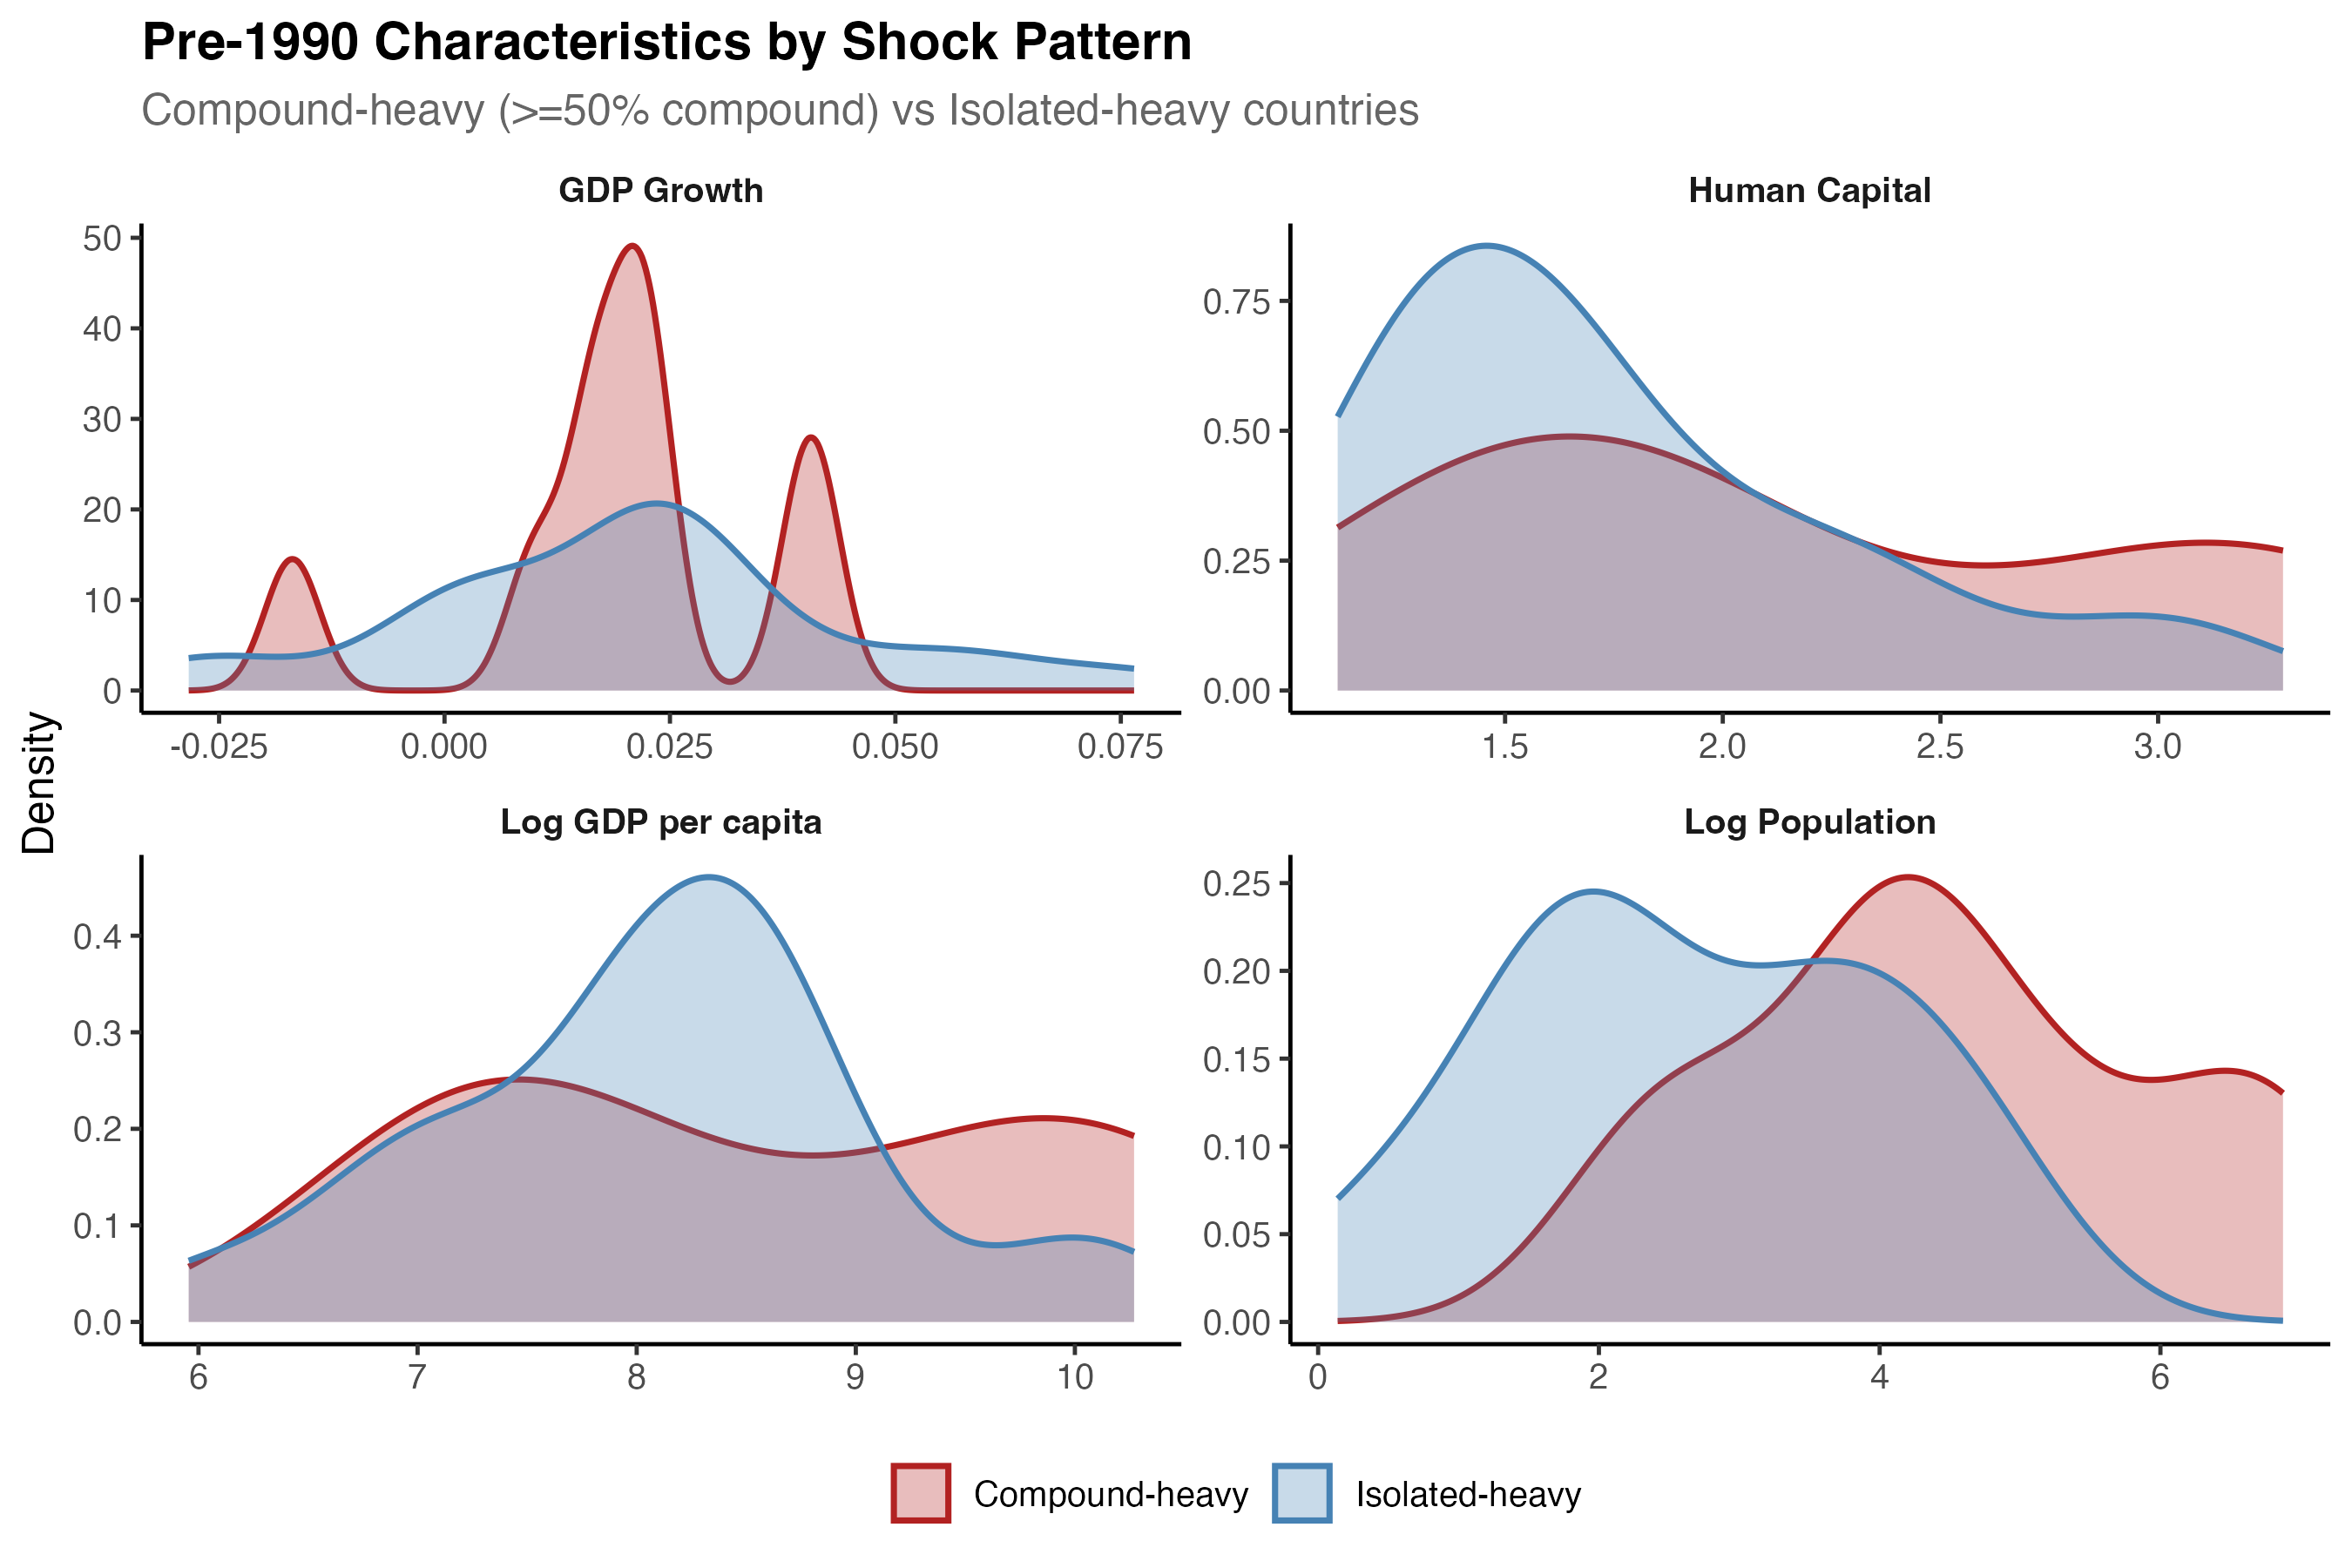
\includegraphics[width=0.72\textwidth,height=0.55\textheight,keepaspectratio]{figures/chars_by_shock_type.png}

\smallskip
\small
Compound-heavy countries are larger (log pop 4.5 vs 2.7), slightly richer, and have higher human capital. These are the large, frequently-hit economies (CHN, JPN, USA). Isolated-heavy countries are smaller Caribbean/Central American nations.
\end{frame}

\begin{frame}{Identification Strategy}
We address the selection problem through:
\begin{enumerate}
  \item \textbf{Within-country variation}: Country FE + country-specific trends ensure we compare compound vs isolated shocks \emph{within the same country's trajectory}
  \item \textbf{Multiple FE specifications}: Year FE, region$\times$year FE
  \item \textbf{Controls}: Lagged GDP growth and lagged shocks absorb autoregressive dynamics
  \item \textbf{Robustness}: Dropping always-compound countries, alternative definitions, continuous intensity
\end{enumerate}

\medskip
\textbf{LP specification}:
\[
  y_{i,t+h} - y_{i,t-1} = \beta_{\text{iso}} \cdot \mathit{Isolated}_{it} + \beta_{\text{comp}} \cdot \mathit{Compound}_{it} + \gamma'X_{it} + \alpha_{i}(t) + \delta_t + \varepsilon_{it}
\]
where $\alpha_i(t)$ includes country-specific linear and quadratic trends.
\end{frame}

% ===============================================================
\section{Main Results}
% ===============================================================

{\hideframenumber
\begin{frame}
\sectionpage
\end{frame}
\showframenumber}

\begin{frame}{Main Result: Interaction Approach}
\centering
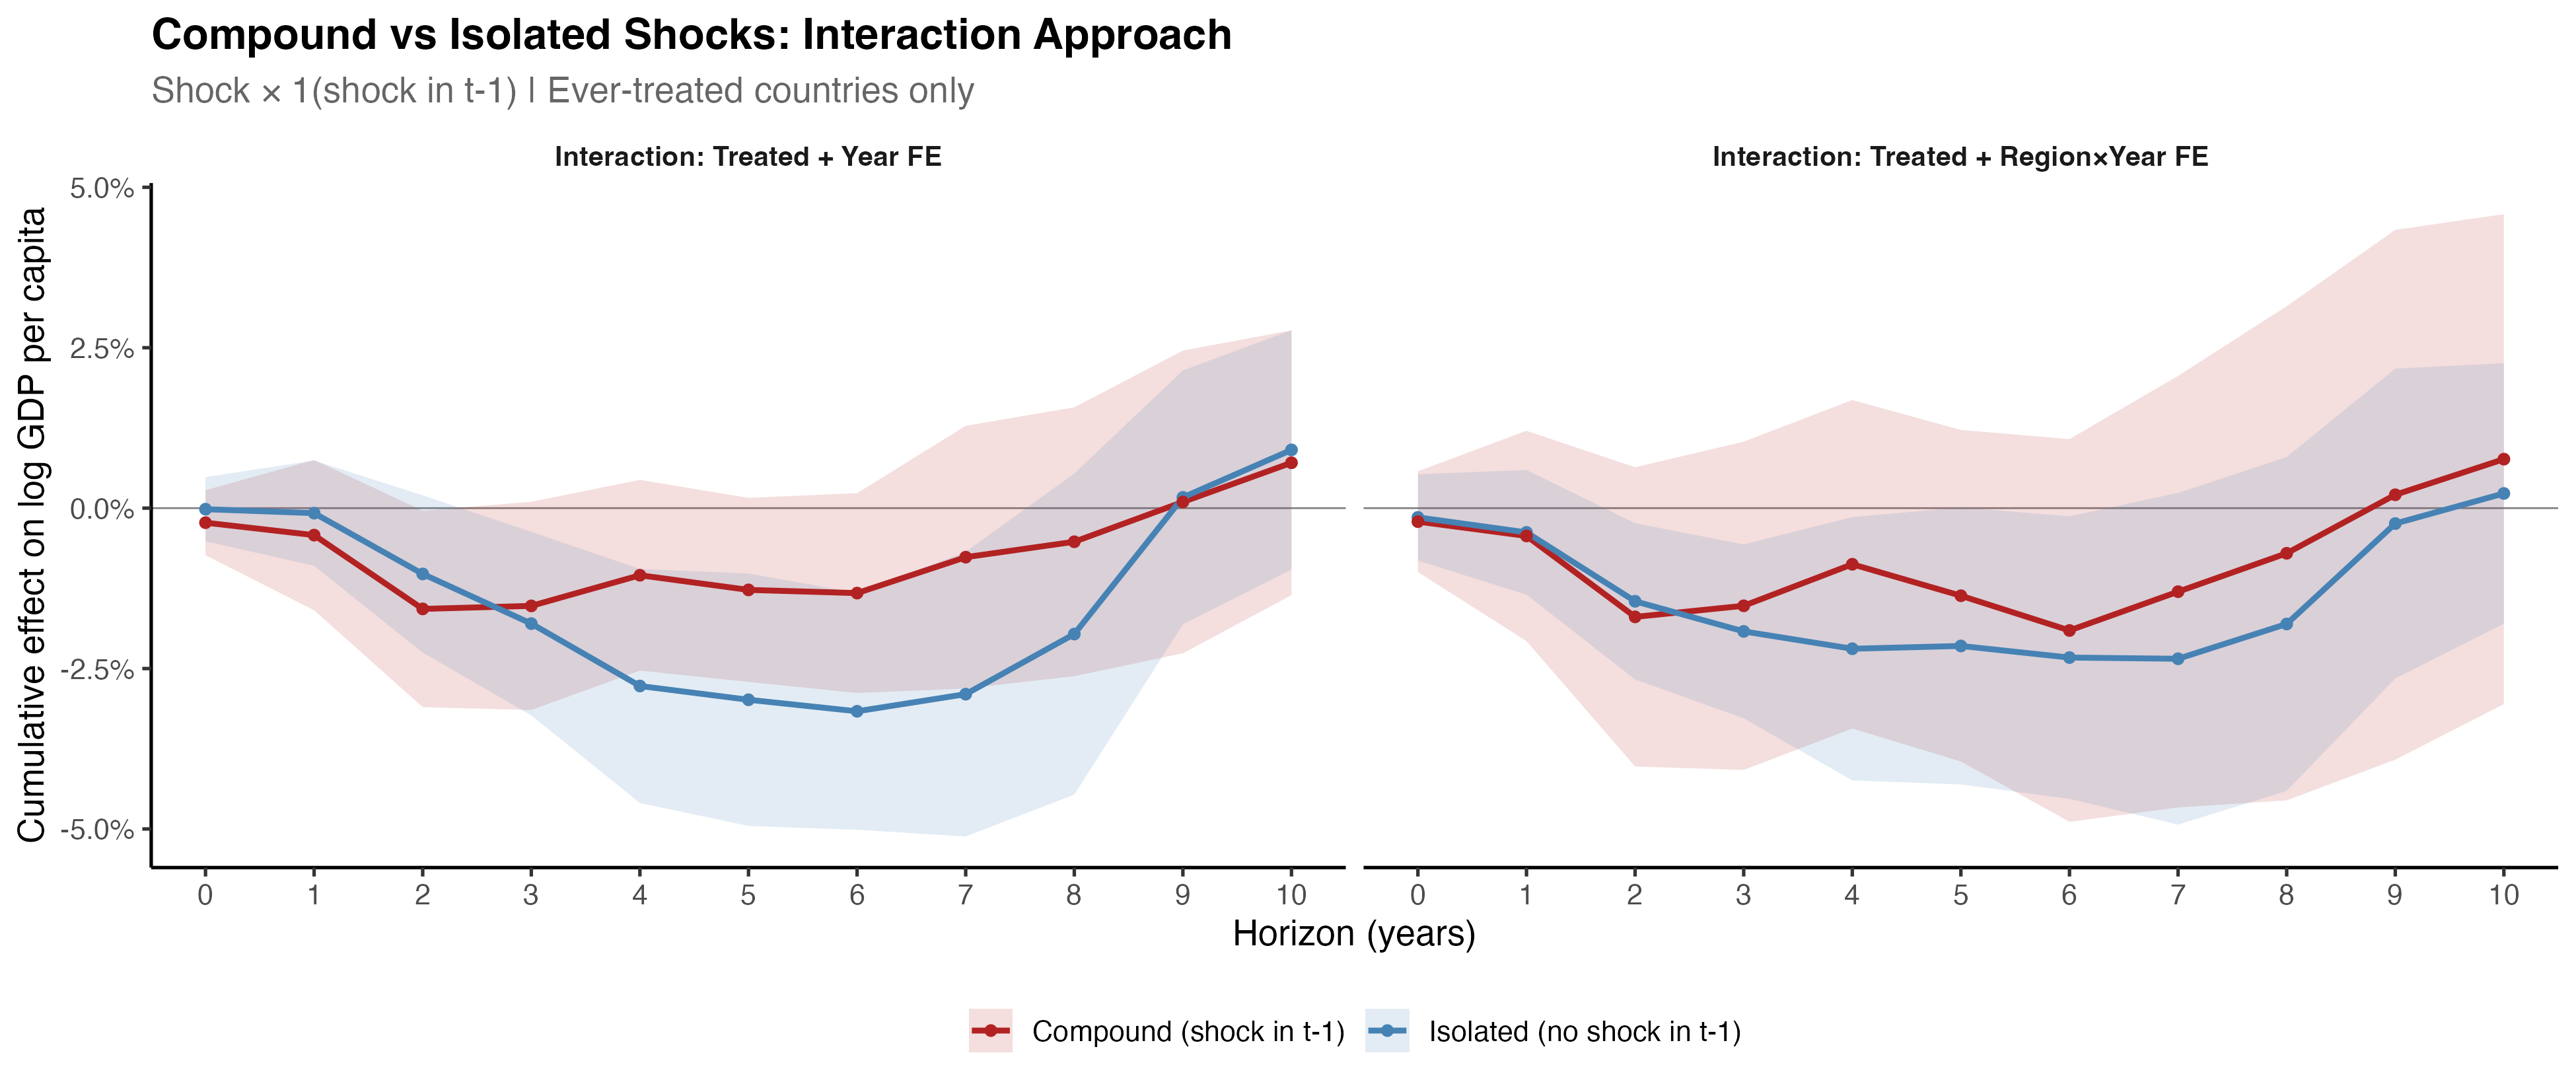
\includegraphics[width=\textwidth,height=0.62\textheight,keepaspectratio]{figures/irf_compound_main.png}

\smallskip
\small
Isolated shocks cause a \textbf{persistent 3.0\% GDP decline} at $h = 5$. Compound shocks cause only a \textbf{1.3\% decline} (insignificant). The difference is not statistically significant ($p > 0.10$), but the point estimates diverge from $h = 2$ onward.
\end{frame}

\begin{frame}{Separate Shock Indicators Across FE Specifications}
\centering
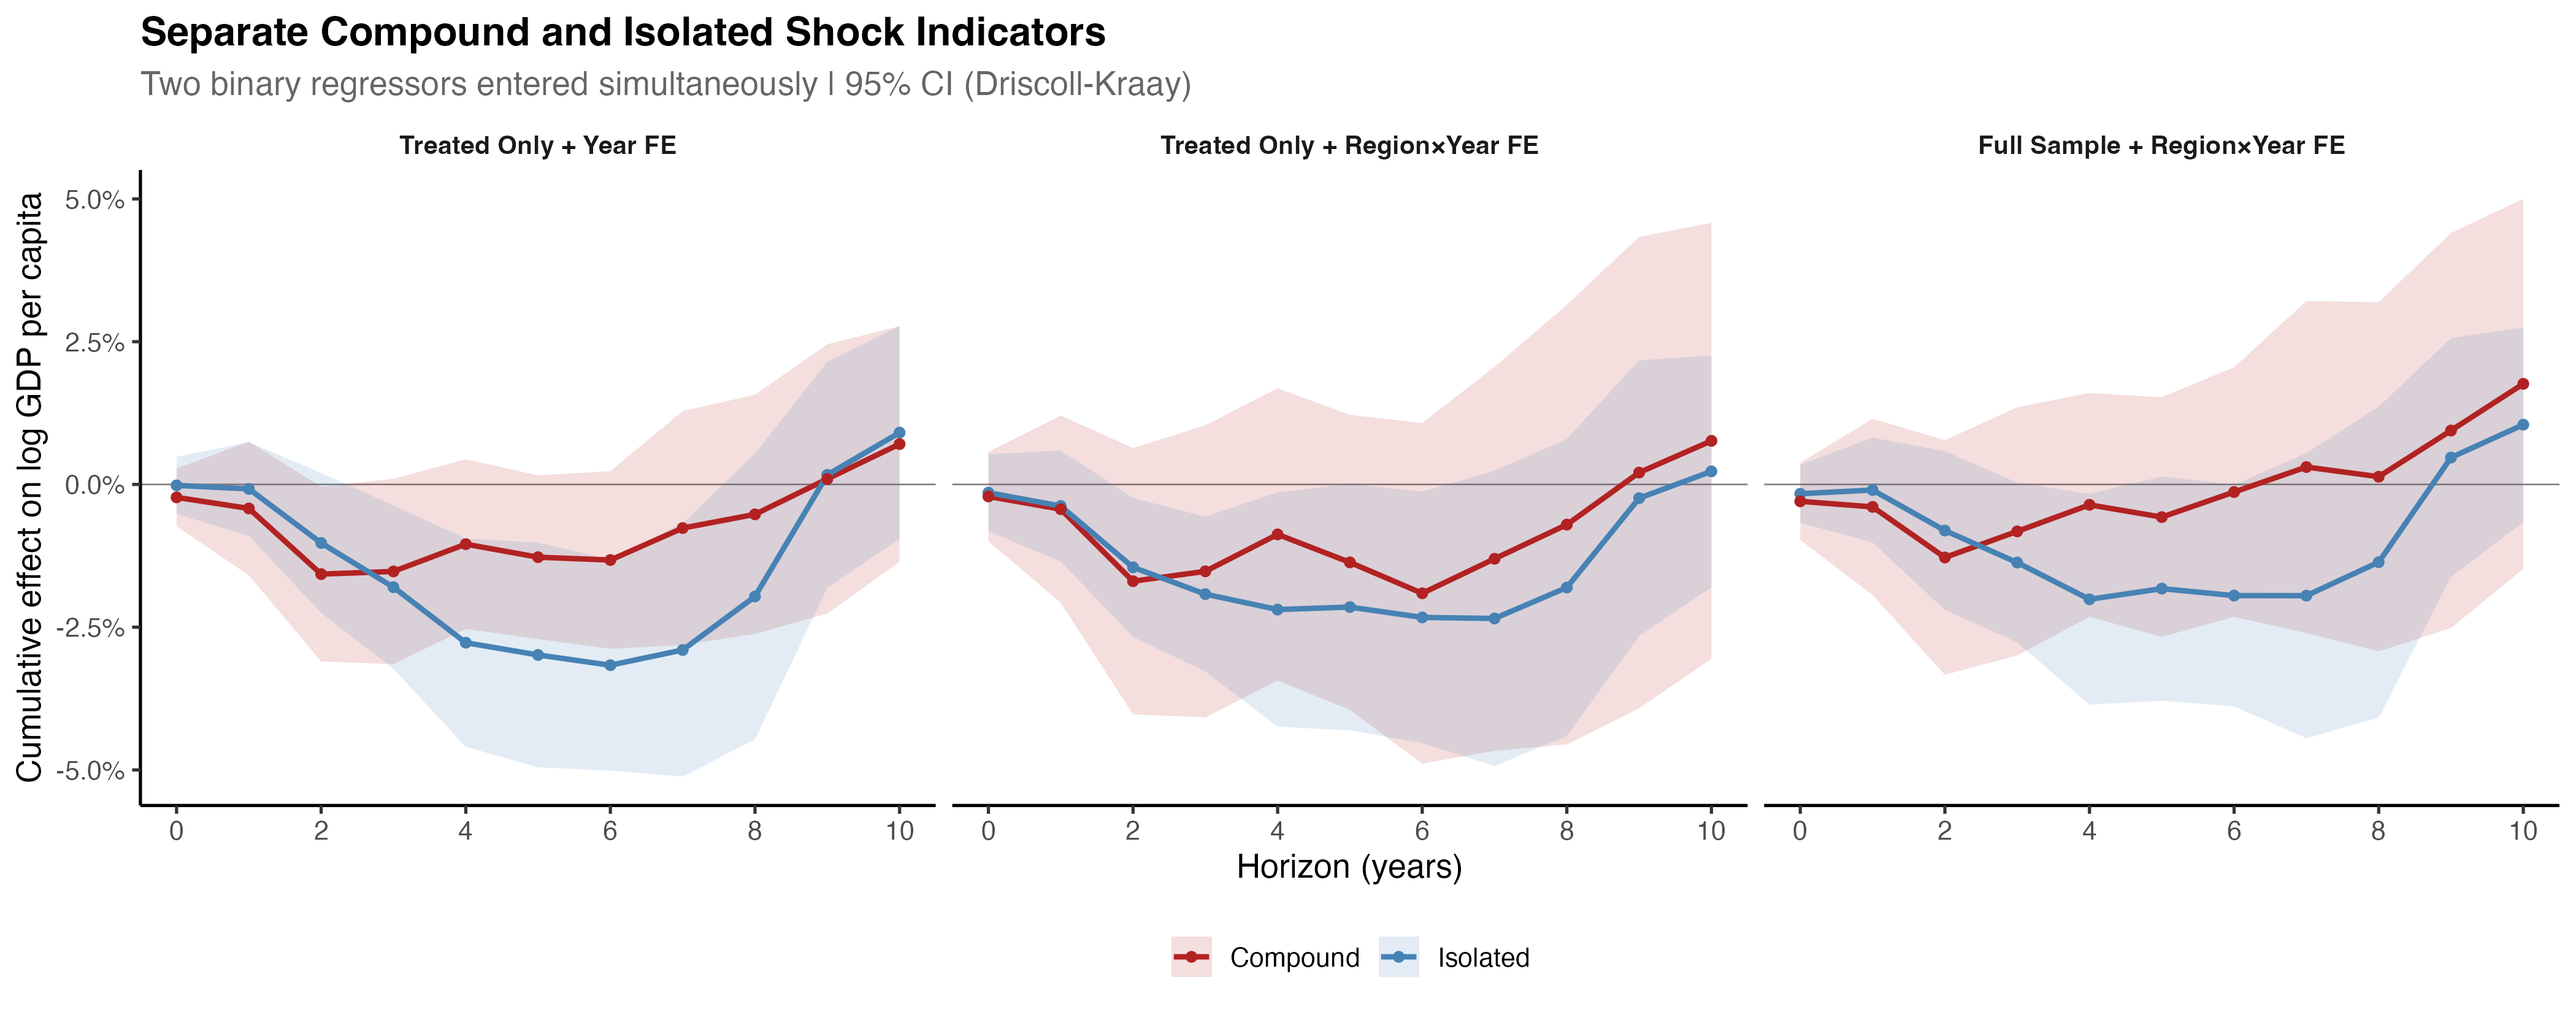
\includegraphics[width=\textwidth,height=0.58\textheight,keepaspectratio]{figures/irf_compound_separate.png}

\smallskip
\small
The pattern is robust to FE specification: isolated shocks are more damaging across all three. Adding never-treated countries as controls (right) or switching to region$\times$year FE (center) does not change the qualitative result.
\end{frame}

\begin{frame}{Compound $-$ Isolated Difference}
\centering
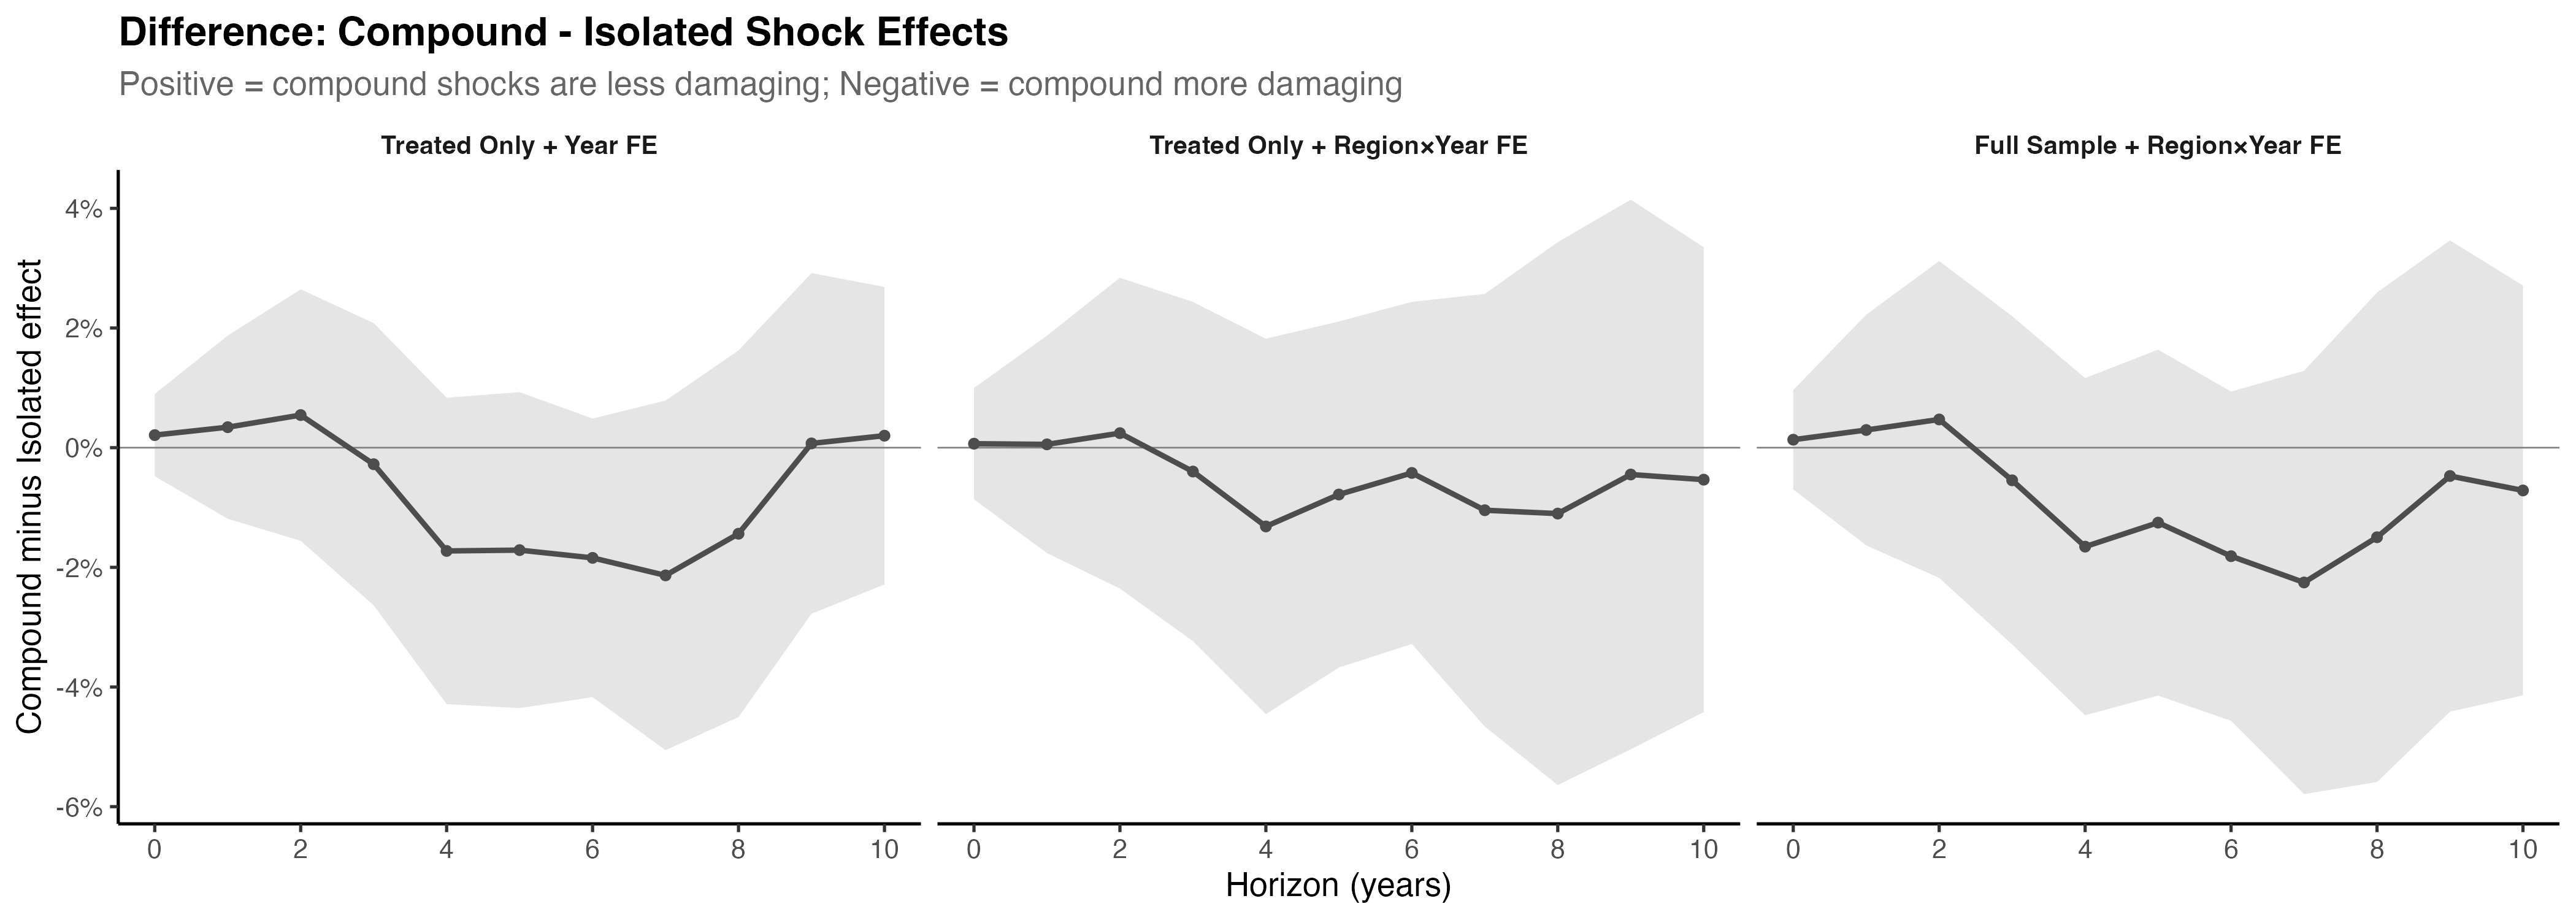
\includegraphics[width=\textwidth,height=0.58\textheight,keepaspectratio]{figures/irf_compound_difference.png}

\smallskip
\small
The difference (compound $-$ isolated) is consistently positive but \textbf{never statistically significant} at 95\%. The wide CIs reflect limited identifying variation: only 19 countries have both types, and the country-specific trends absorb much of the signal.
\end{frame}

\begin{frame}{Results at $h = 5$}
\centering
\begin{tabular}{l r r r}
\hline
\textbf{Specification} & \textbf{Isolated} & \textbf{Compound} & \textbf{Diff} \\
\hline
Treated + Year FE              & $-3.0\%^{**}$  & $-1.3\%$     & $+1.7\%$ \\
Treated + Region$\times$Year FE & $-2.1\%^{*}$  & $-1.4\%$     & $+0.8\%$ \\
Full Sample + Region$\times$Year FE & $-1.8\%^{*}$ & $-0.6\%$ & $+1.3\%$ \\
\hline
\end{tabular}

\bigskip
\begin{itemize}
  \item Isolated shocks consistently larger in magnitude
  \item Compound shocks are smaller and often insignificant
  \item The difference is not statistically significant in any specification
  \item \textbf{Interpretation}: Compound shocks appear \emph{less} damaging than isolated ones --- consistent with diminishing marginal damage, not compounding
\end{itemize}
\end{frame}

% ===============================================================
\section{Robustness}
% ===============================================================

{\hideframenumber
\begin{frame}
\sectionpage
\end{frame}
\showframenumber}

\begin{frame}{Broader Compound Definition: Shock in $t{-}1$ or $t{-}2$}
\centering
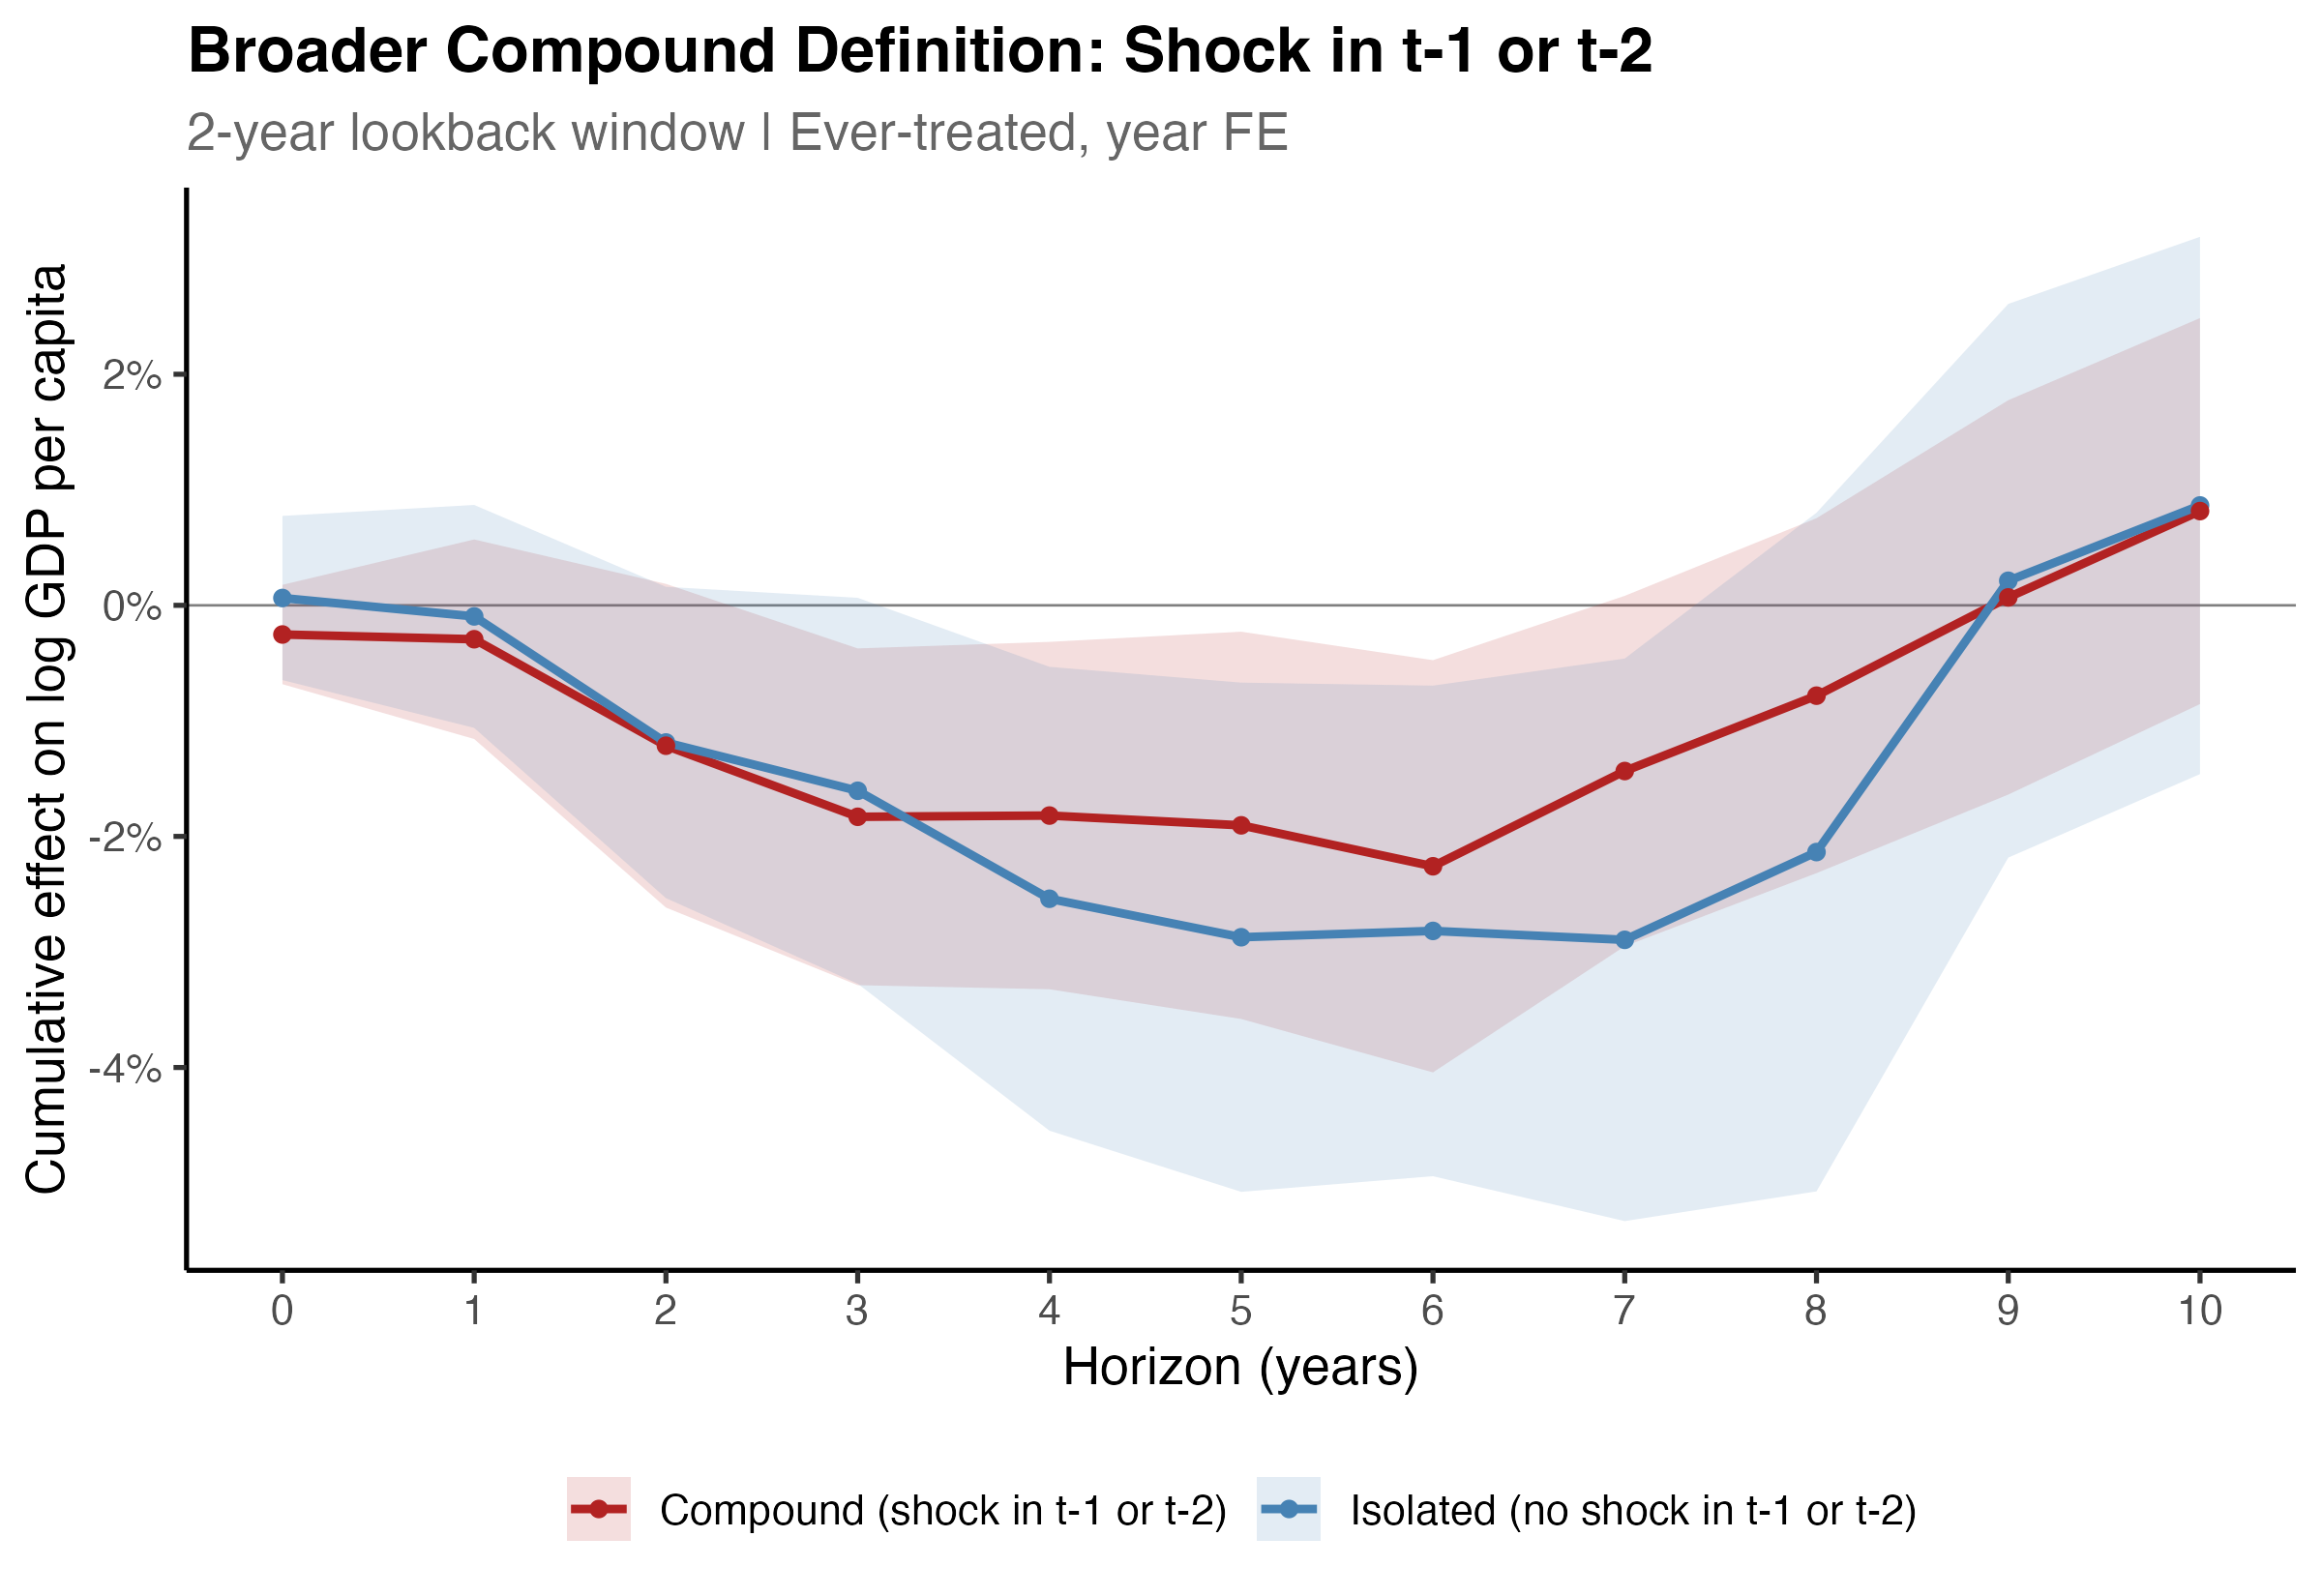
\includegraphics[width=0.72\textwidth,height=0.58\textheight,keepaspectratio]{figures/irf_broad_compound.png}

\smallskip
\small
Extending the lookback window to 2 years: the pattern is similar. Isolated shocks (no shock in $t{-}1$ or $t{-}2$) are more damaging, but the gap narrows because some previously-isolated shocks are reclassified as compound.
\end{frame}

\begin{frame}{Cumulative Exposure: 0, 1, or 2+ Shocks in Past 3 Years}
\centering
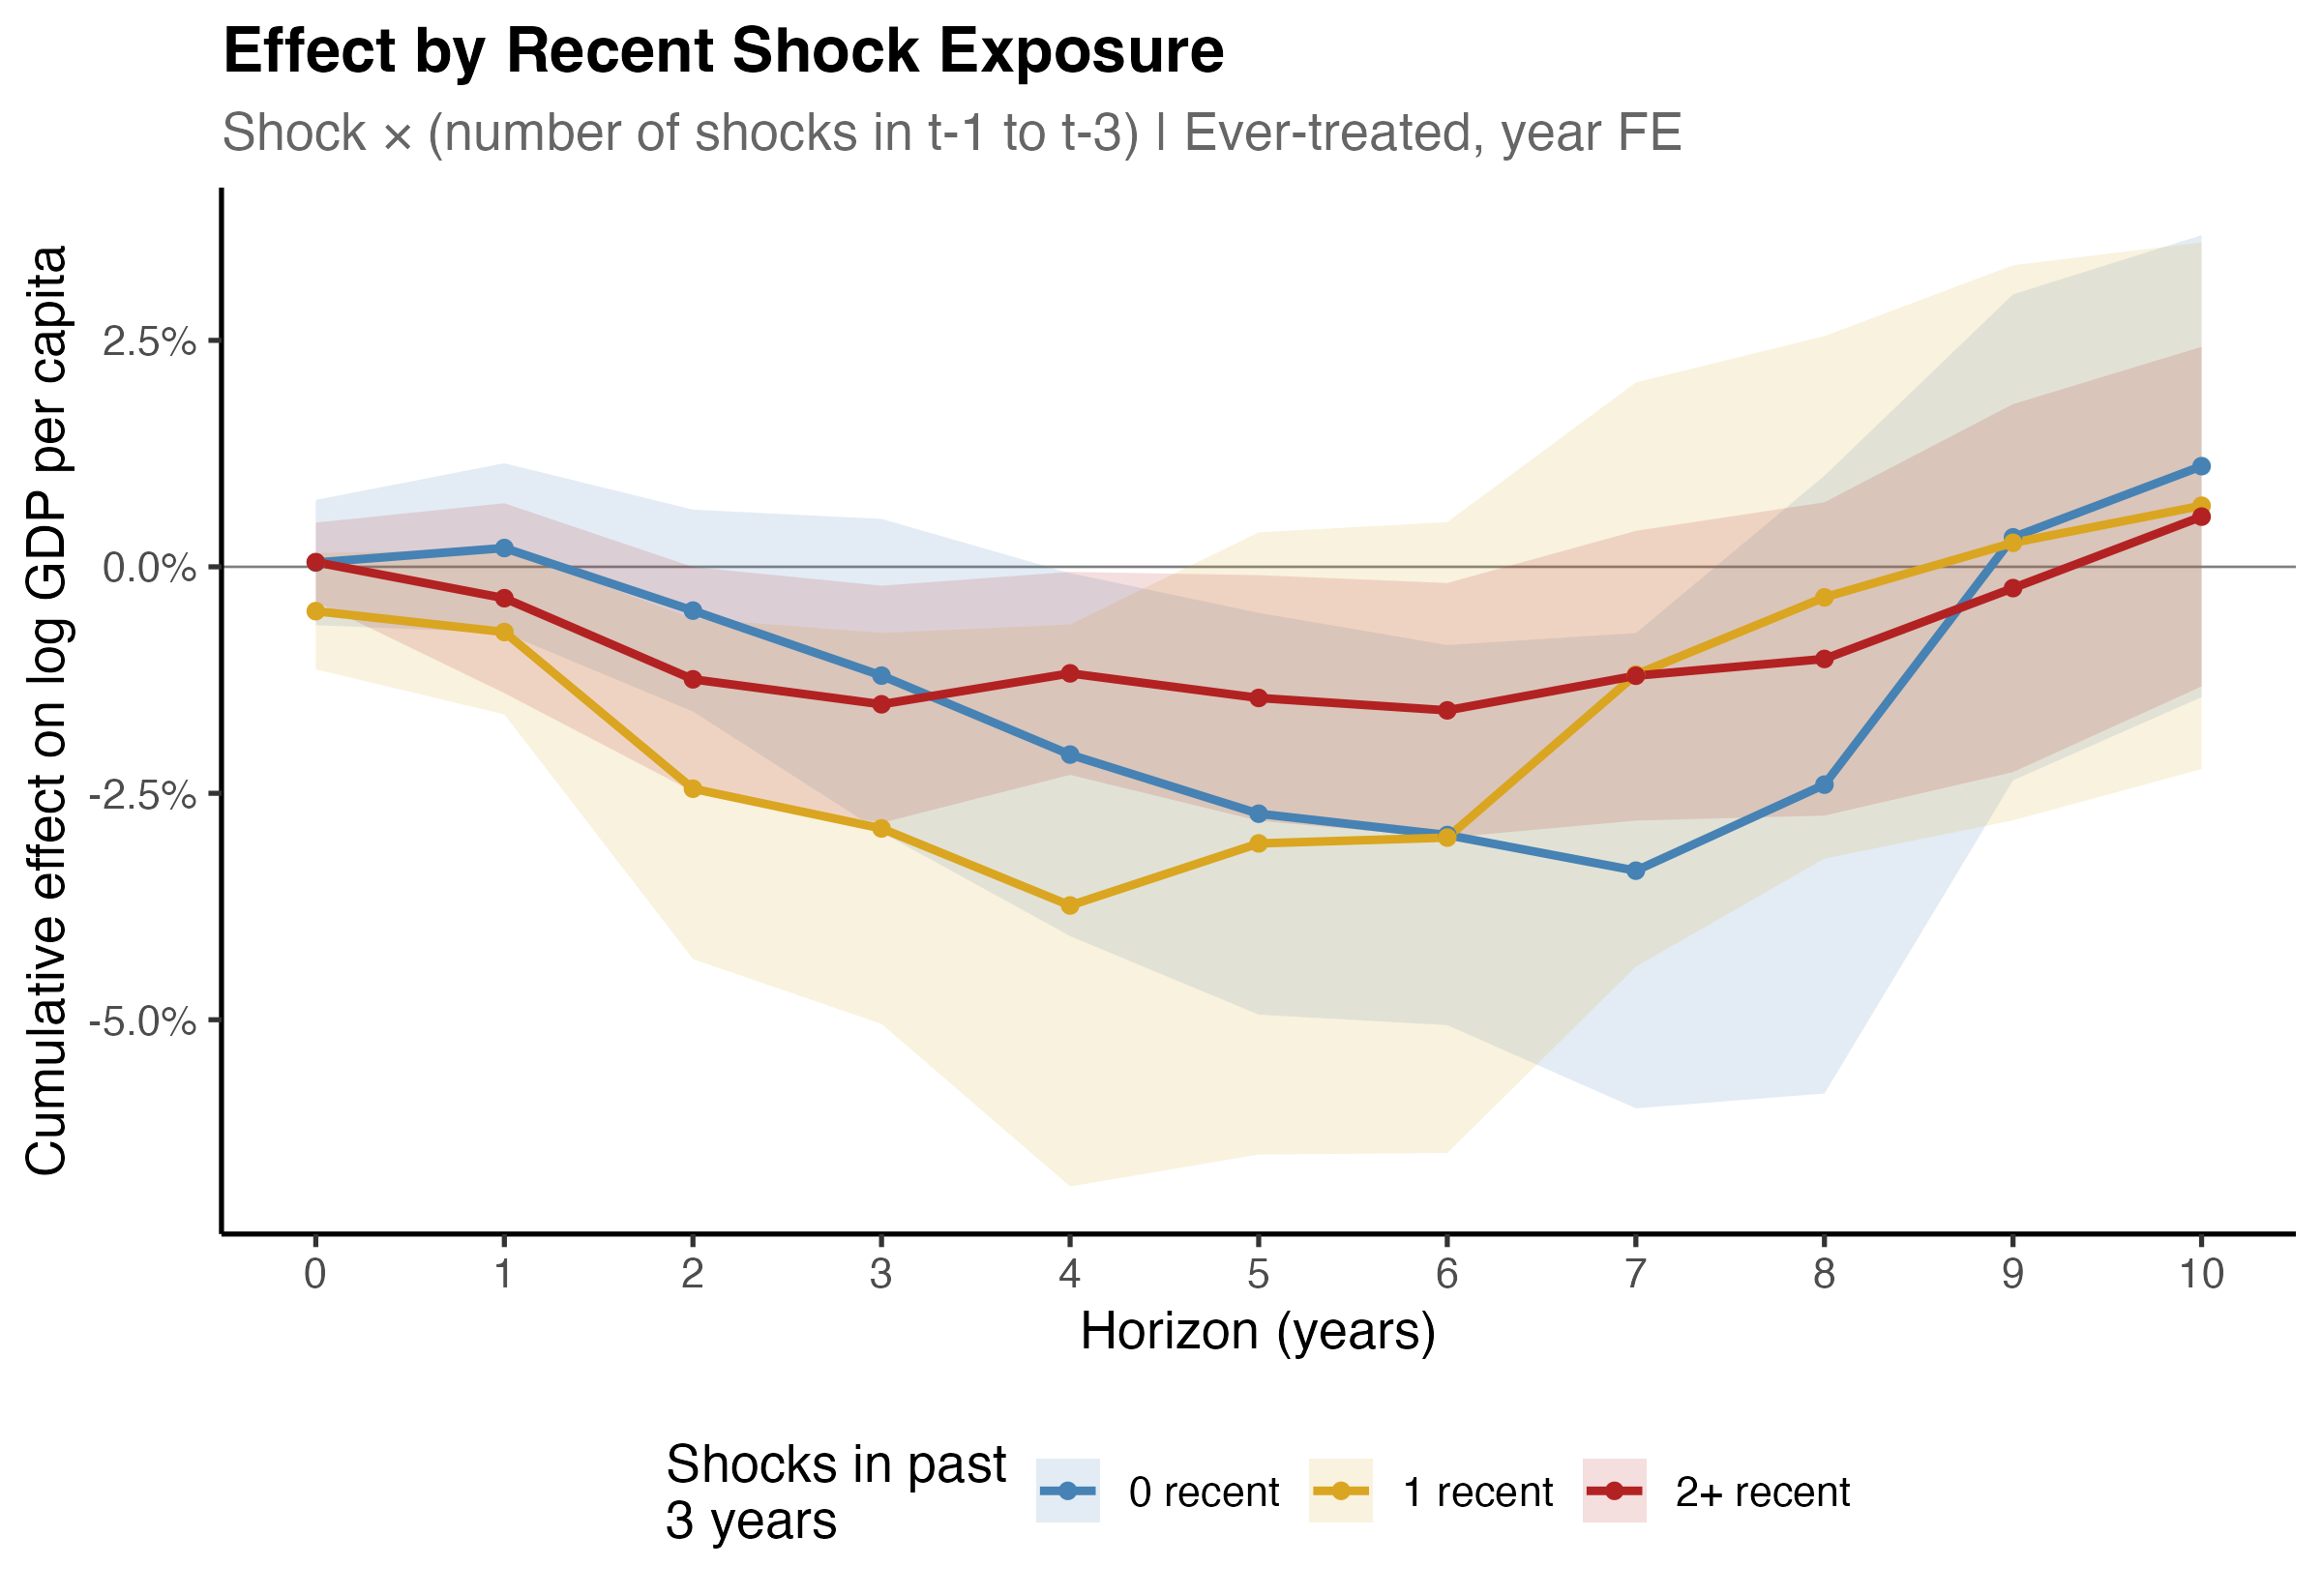
\includegraphics[width=0.72\textwidth,height=0.58\textheight,keepaspectratio]{figures/irf_cumulative_exposure.png}

\smallskip
\small
The dose-response is \textbf{non-monotonic}: 0 and 1 recent shocks produce similar damage ($-2.7\%$ and $-3.1\%$), while 2+ recent shocks produce \emph{less} damage ($-1.4\%$). This is consistent with diminishing marginal effects at high exposure.
\end{frame}

\begin{frame}{Dropping Always-Compound Countries}
\centering
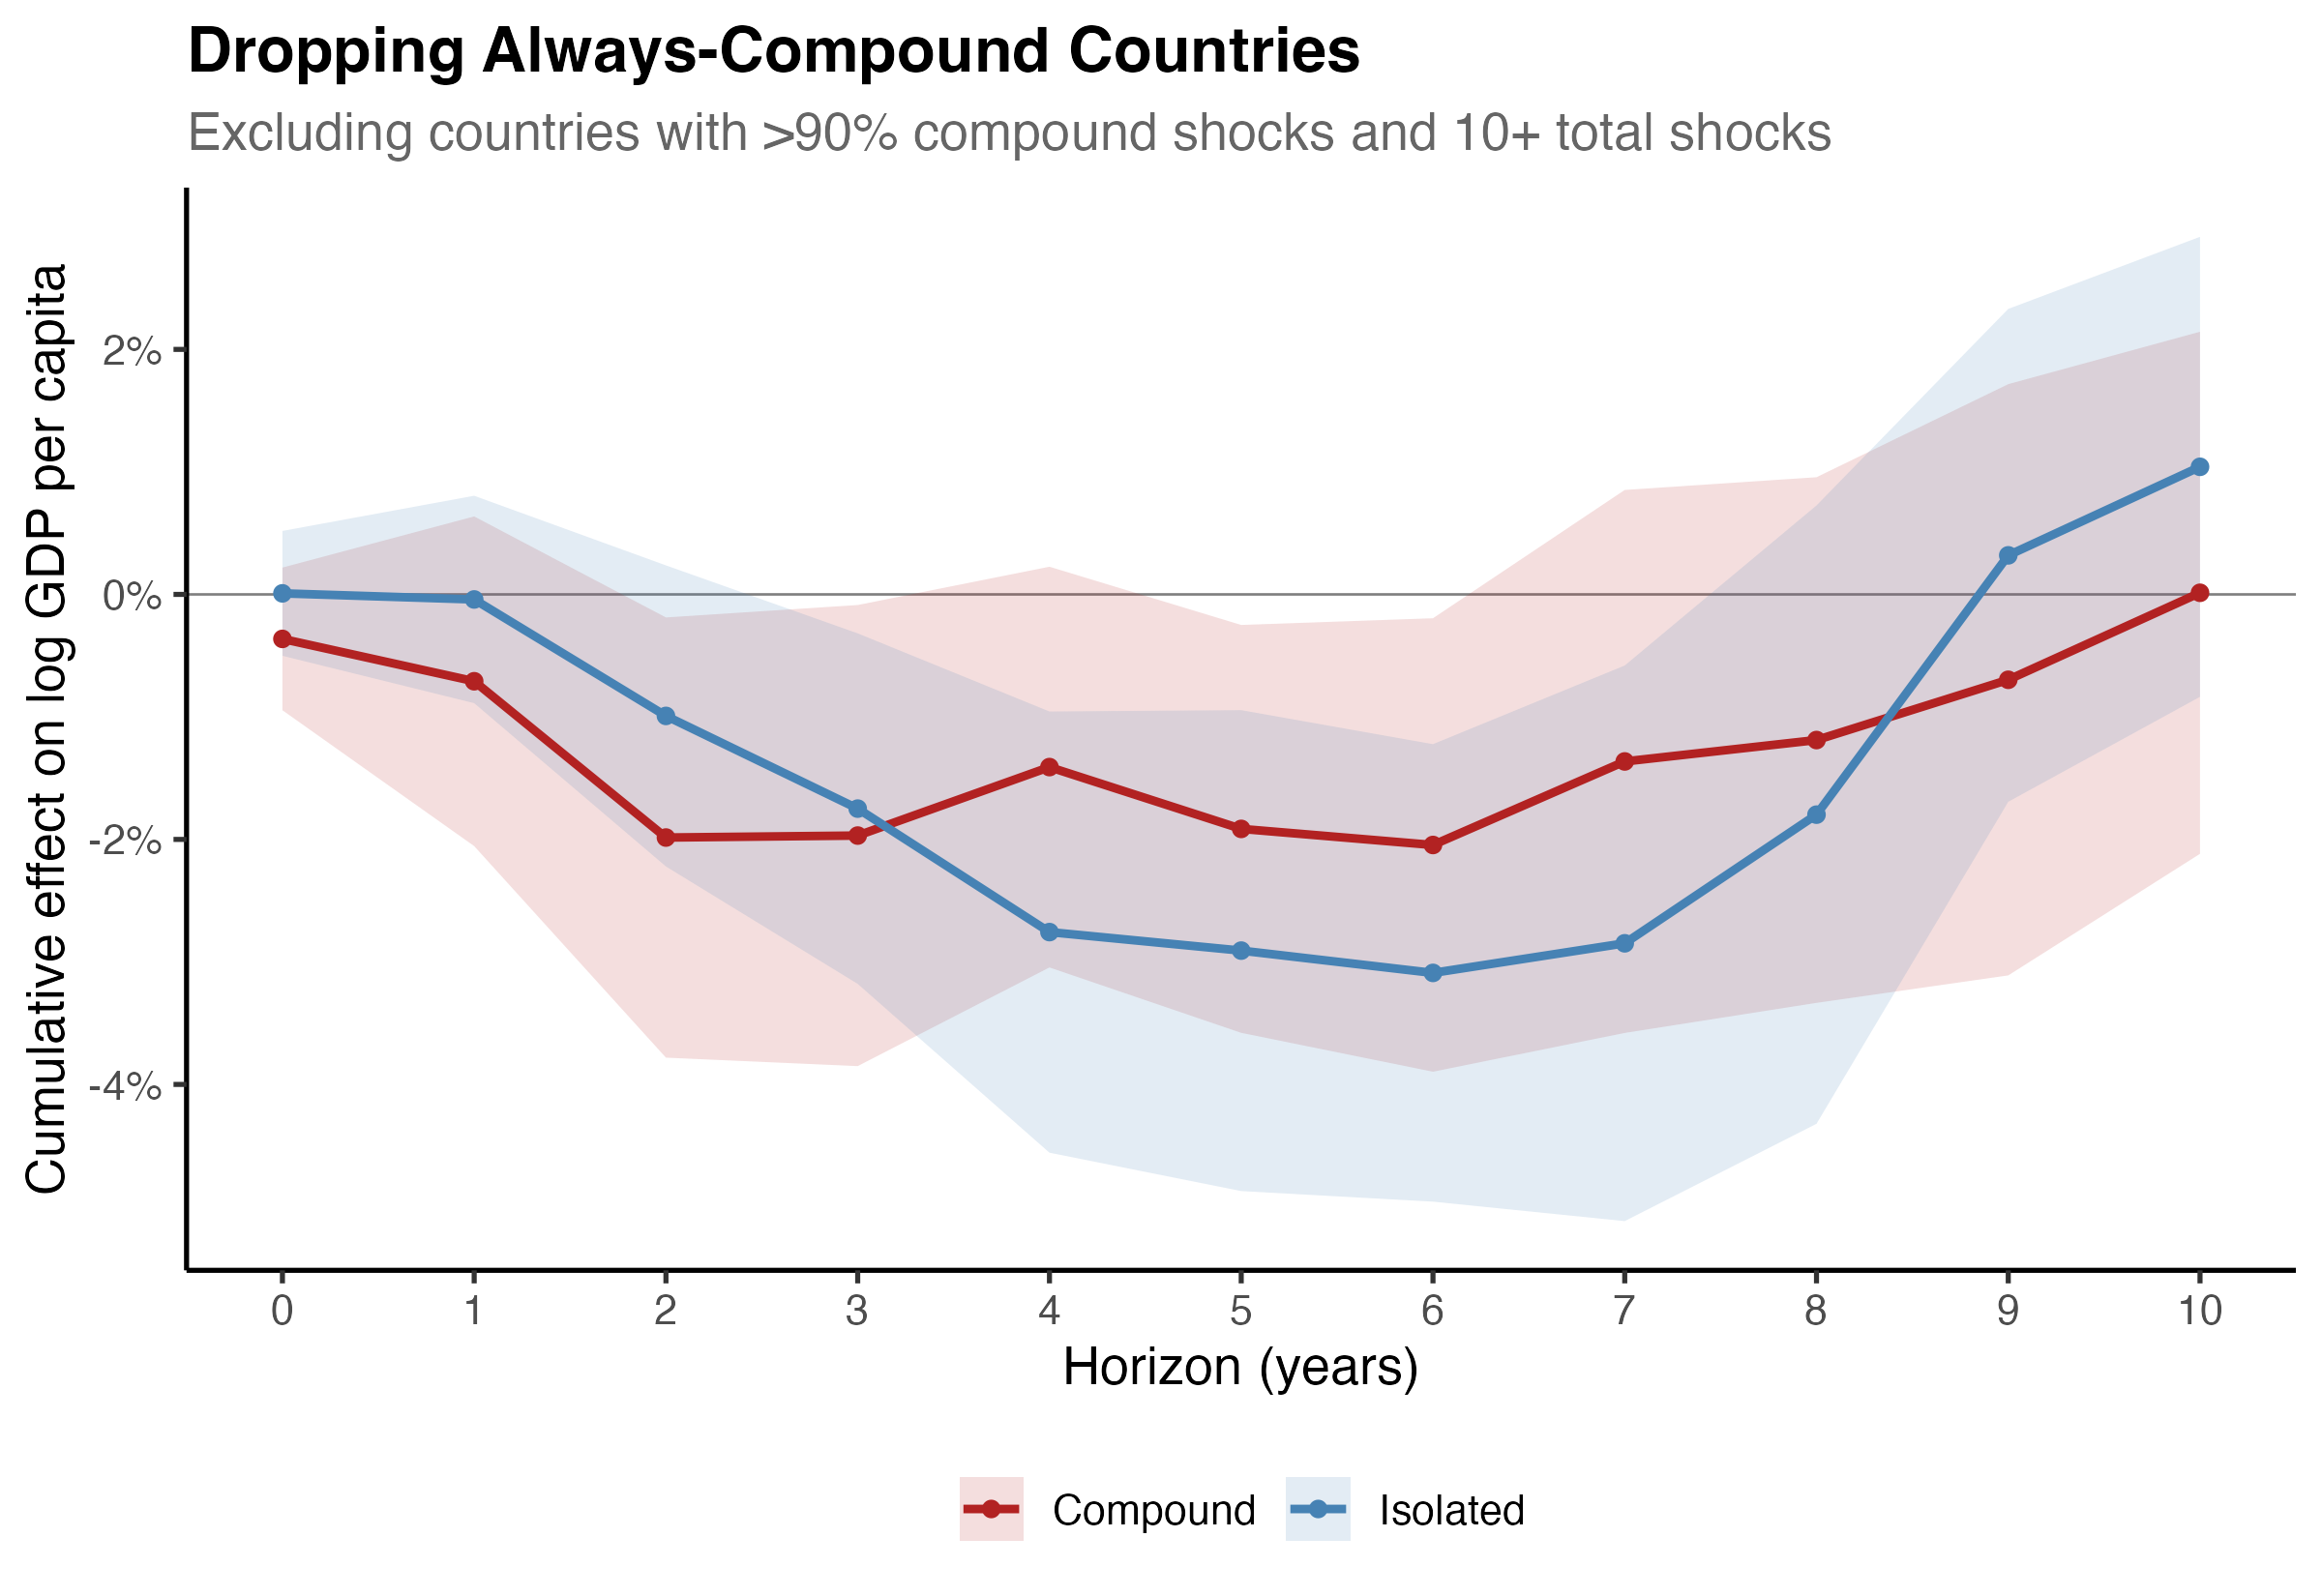
\includegraphics[width=0.72\textwidth,height=0.58\textheight,keepaspectratio]{figures/irf_drop_always_compound.png}

\smallskip
\small
Dropping the 3 countries with $\geq 90\%$ compound shocks and $\geq 10$ total shocks (CHN, PHL, AUS): the pattern persists. Isolated shocks: $-2.9\%$; compound: $-1.9\%$. This addresses the concern that the result is driven by these large, frequently-hit economies.
\end{frame}

\begin{frame}{Continuous Wind Speed $\times$ Recent Shock}
\centering
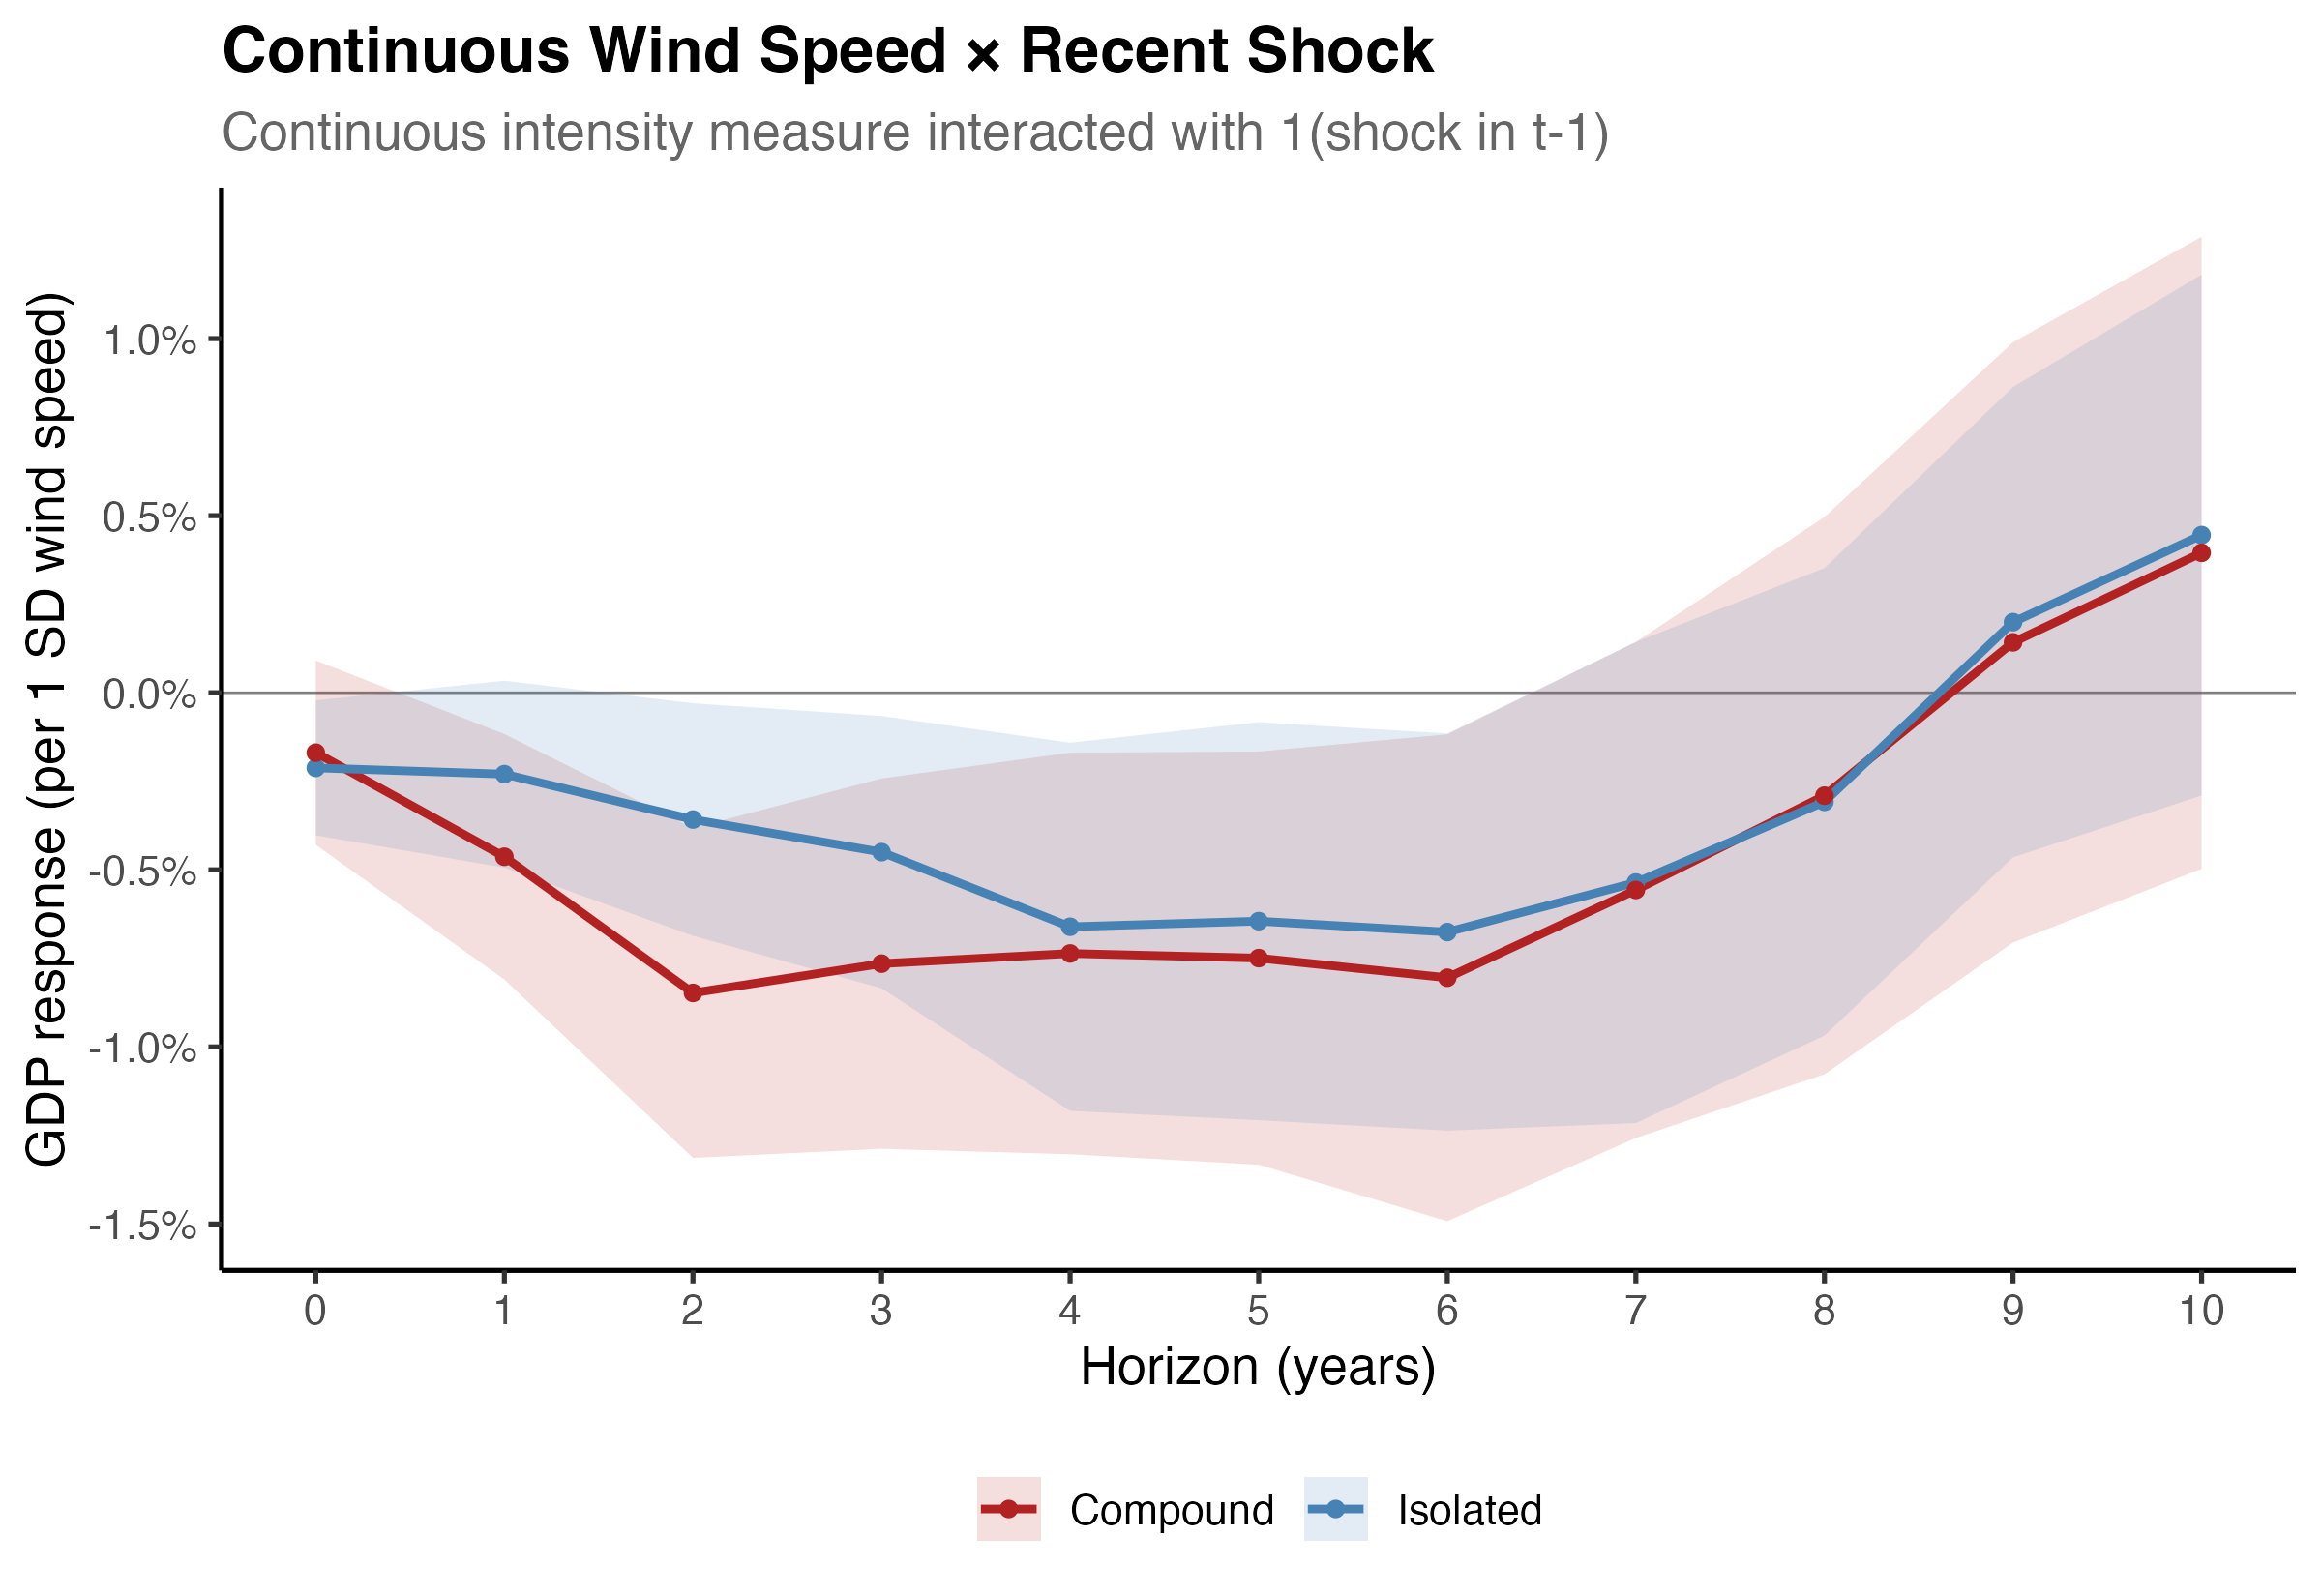
\includegraphics[width=0.72\textwidth,height=0.58\textheight,keepaspectratio]{figures/irf_continuous_compound.png}

\smallskip
\small
Using continuous wind speed (per 1 SD) instead of the binary indicator: the compound/isolated difference \textbf{disappears}. Both are $\approx -0.6\%$ to $-0.7\%$ per SD. The binary result may partly reflect intensity differences between compound and isolated shocks.
\end{frame}

\begin{frame}{Compound $\times$ Period Interaction}
\centering
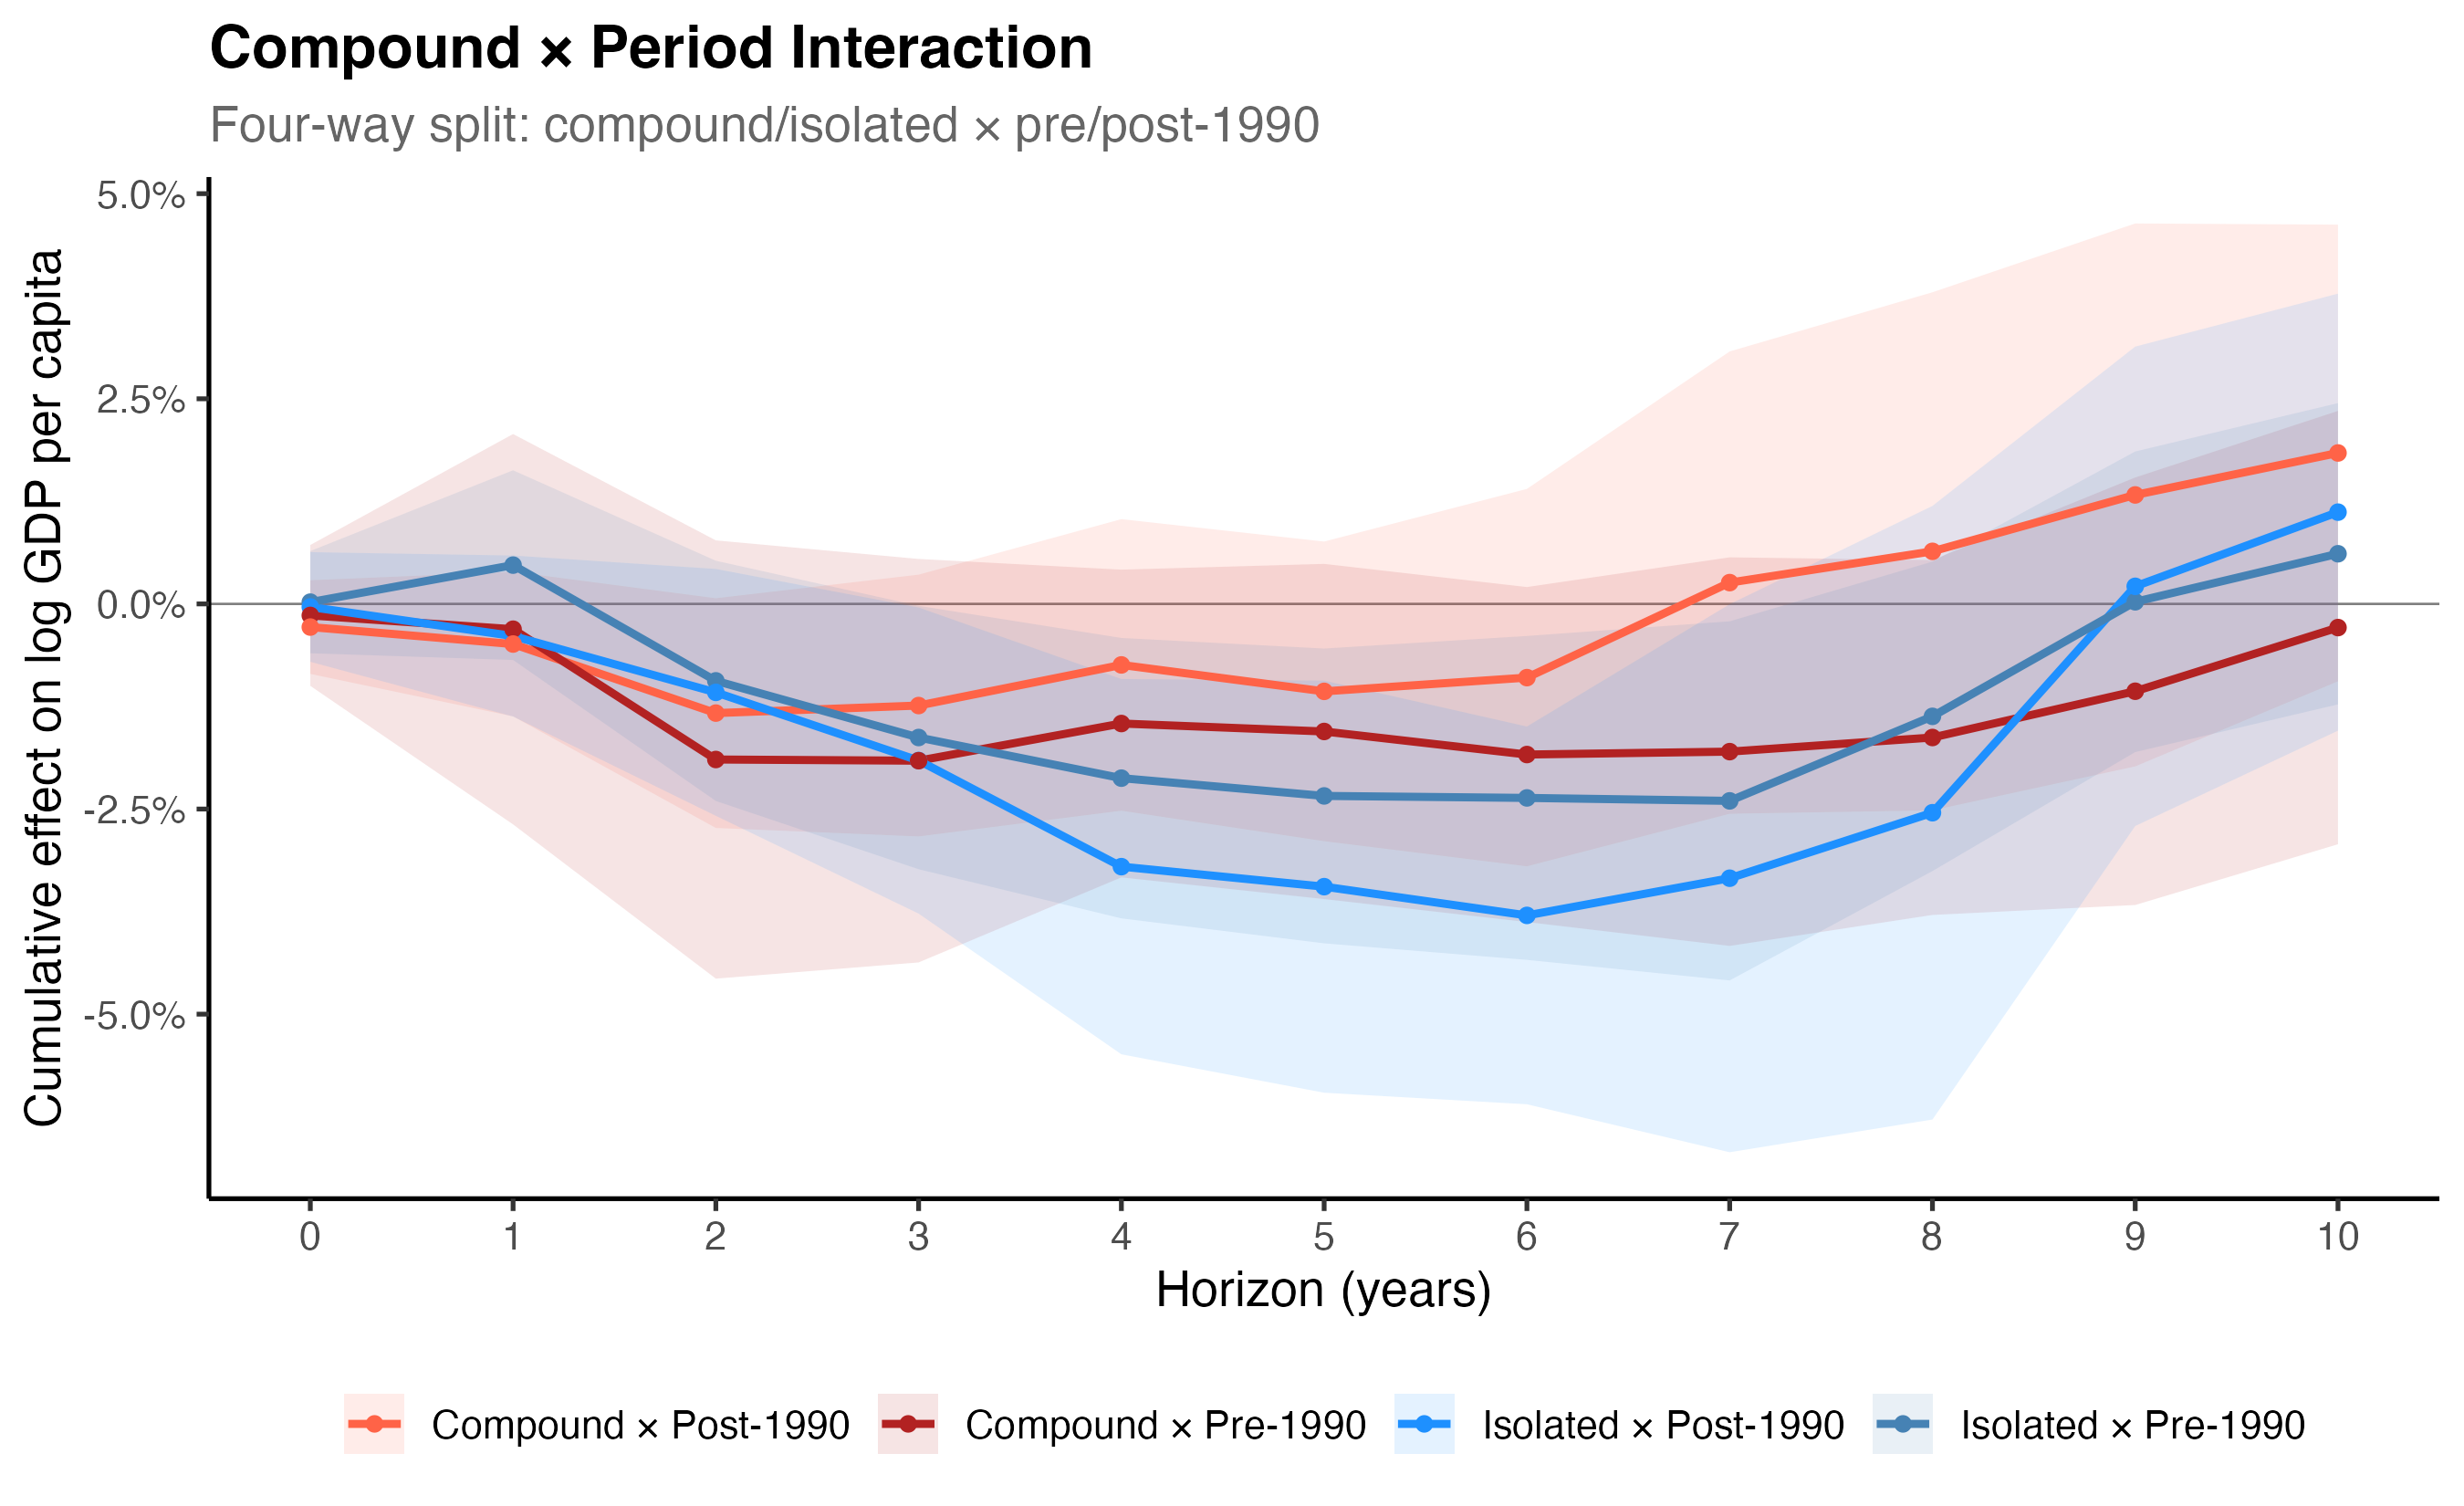
\includegraphics[width=0.72\textwidth,height=0.60\textheight,keepaspectratio]{figures/irf_compound_period.png}

\smallskip
\small
Four-way split: Isolated post-1990 shocks are most damaging ($-3.4\%$). Compound shocks are attenuated in both periods. The compound/isolated gap does not widen post-1990 --- the period divergence in the main analysis operates through a different channel.
\end{frame}

\begin{frame}{Country + Year FE Only (No Trends)}
\centering
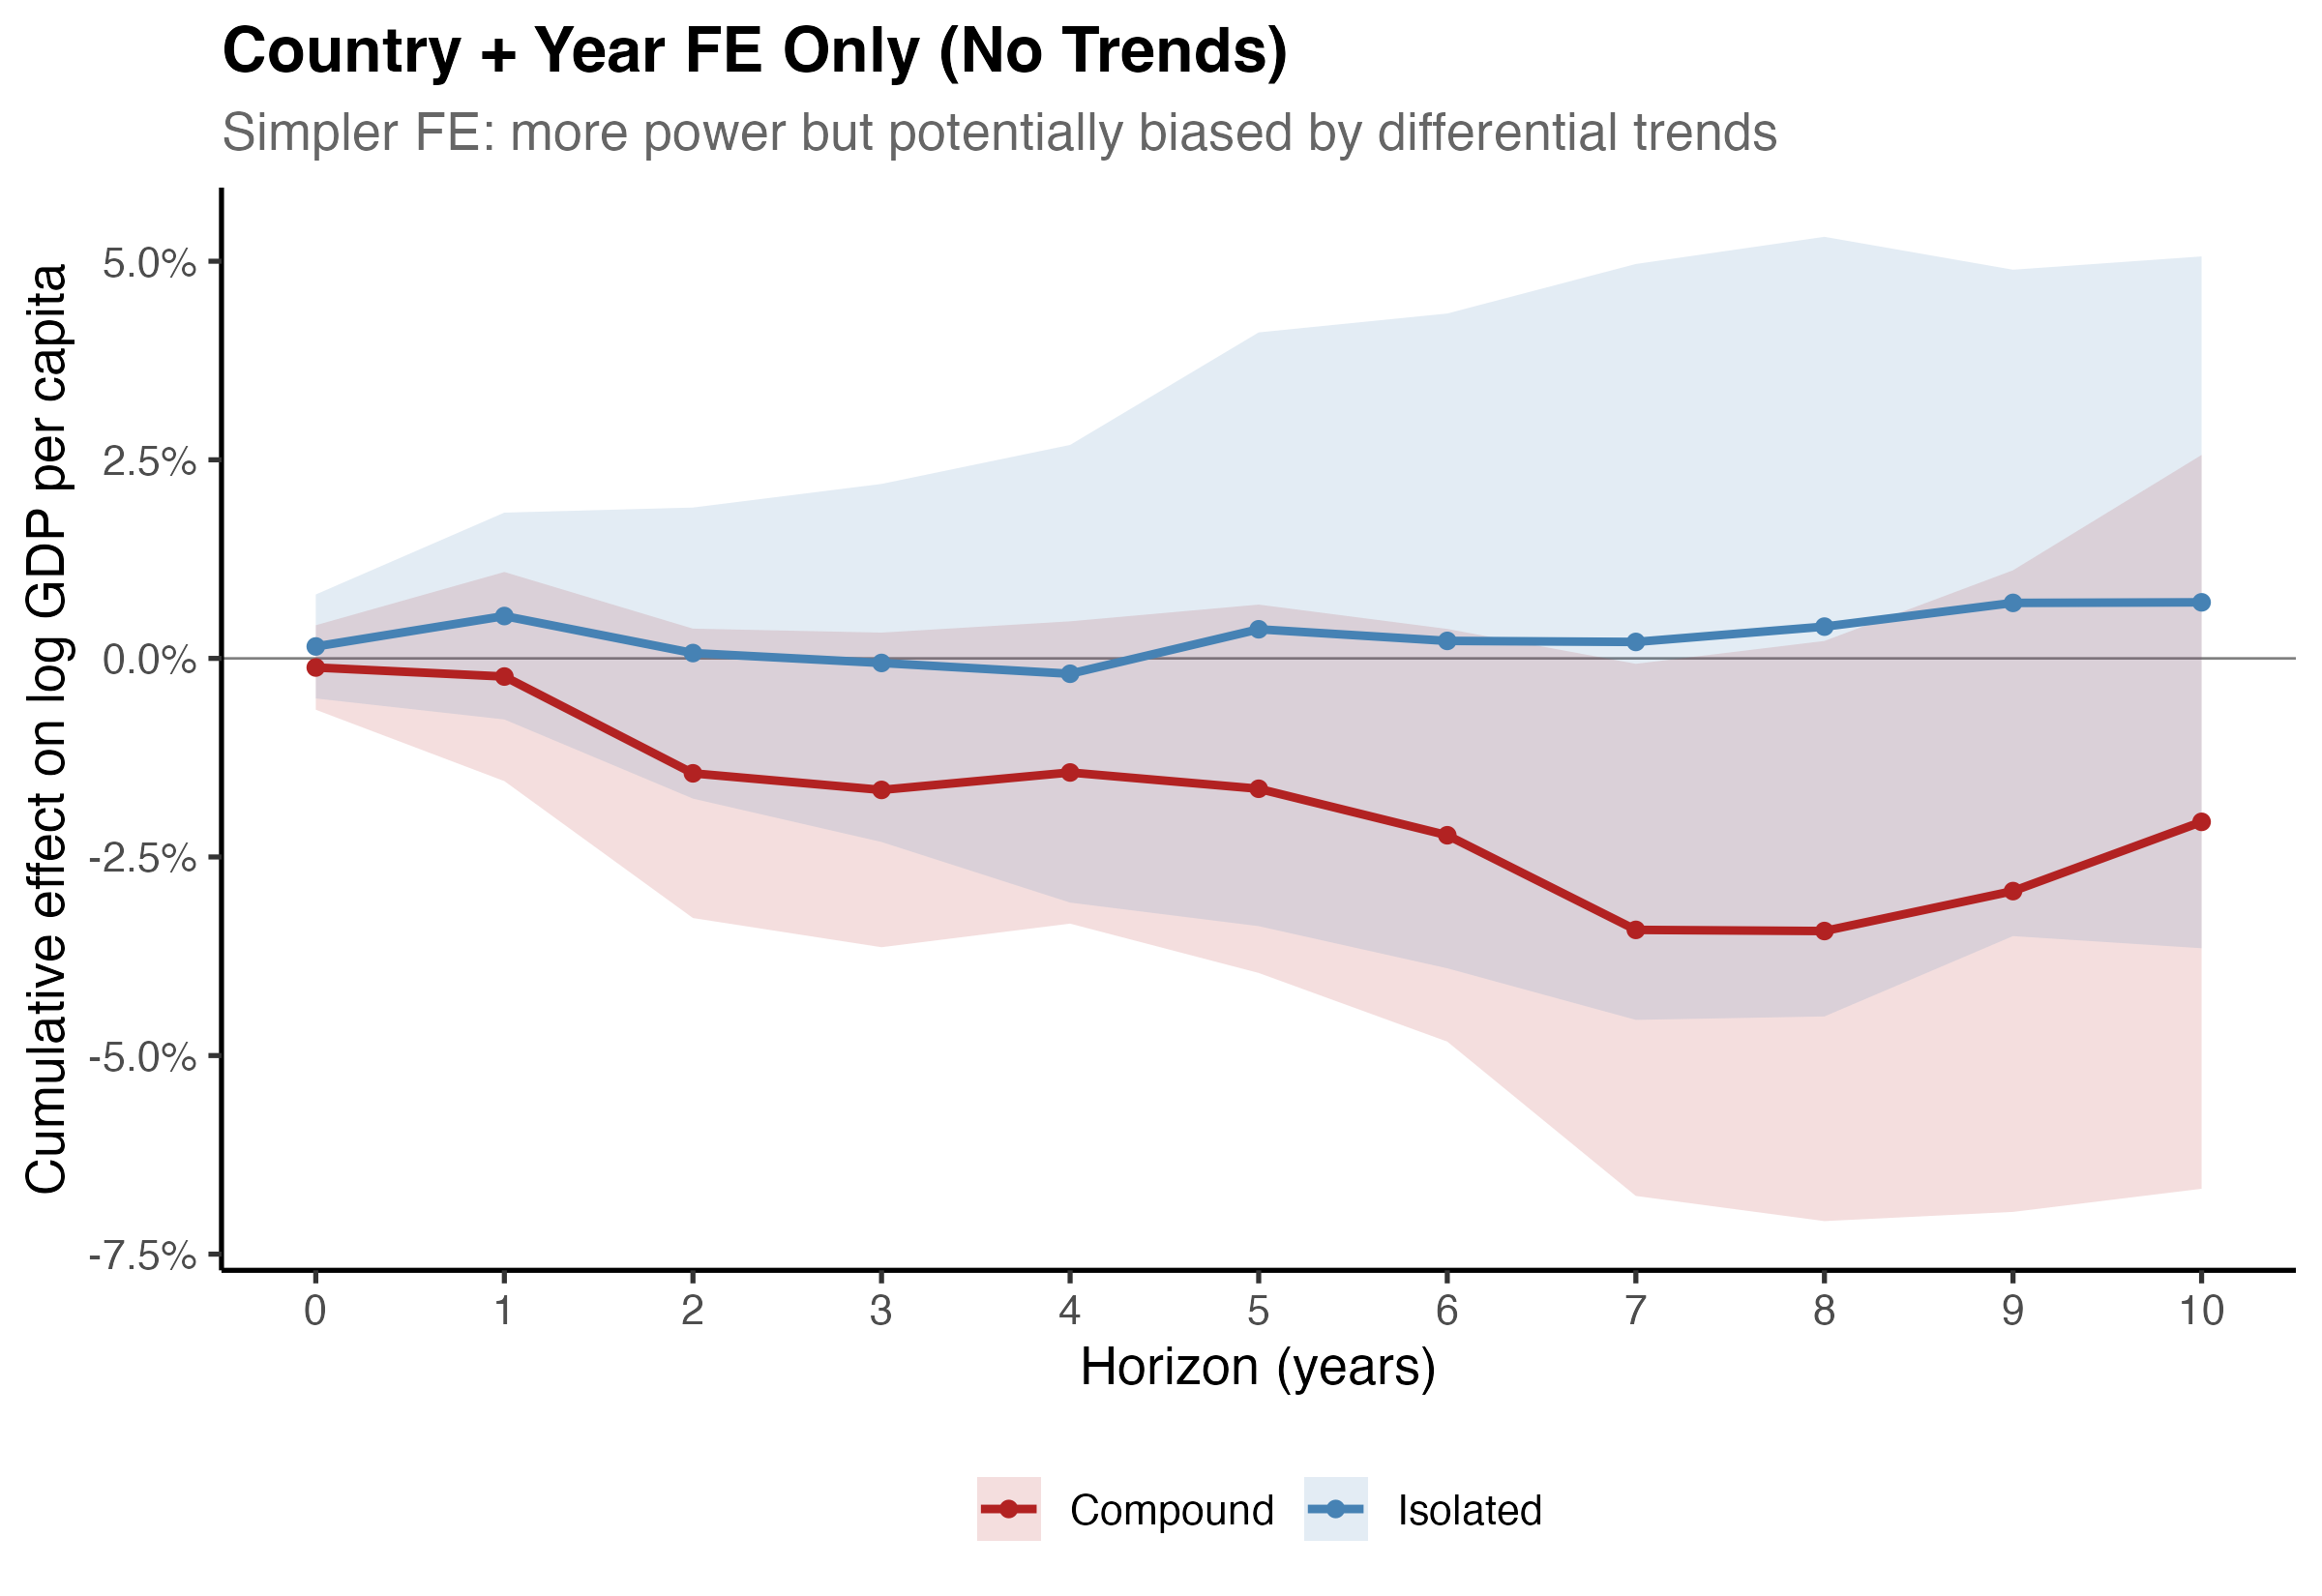
\includegraphics[width=0.72\textwidth,height=0.58\textheight,keepaspectratio]{figures/irf_no_trends.png}

\smallskip
\small
Without country-specific polynomial trends (more power, but potentially biased): the isolated effect vanishes and compound flips sign. Country trends are essential --- without them, the LP conflates the shock effect with differential growth paths of frequently vs.\ infrequently hit countries.
\end{frame}

% ===============================================================
\section{Varying the Treatment Threshold}
% ===============================================================

{\hideframenumber
\begin{frame}
\sectionpage
\end{frame}
\showframenumber}

\begin{frame}{IRFs Across Thresholds}
\centering
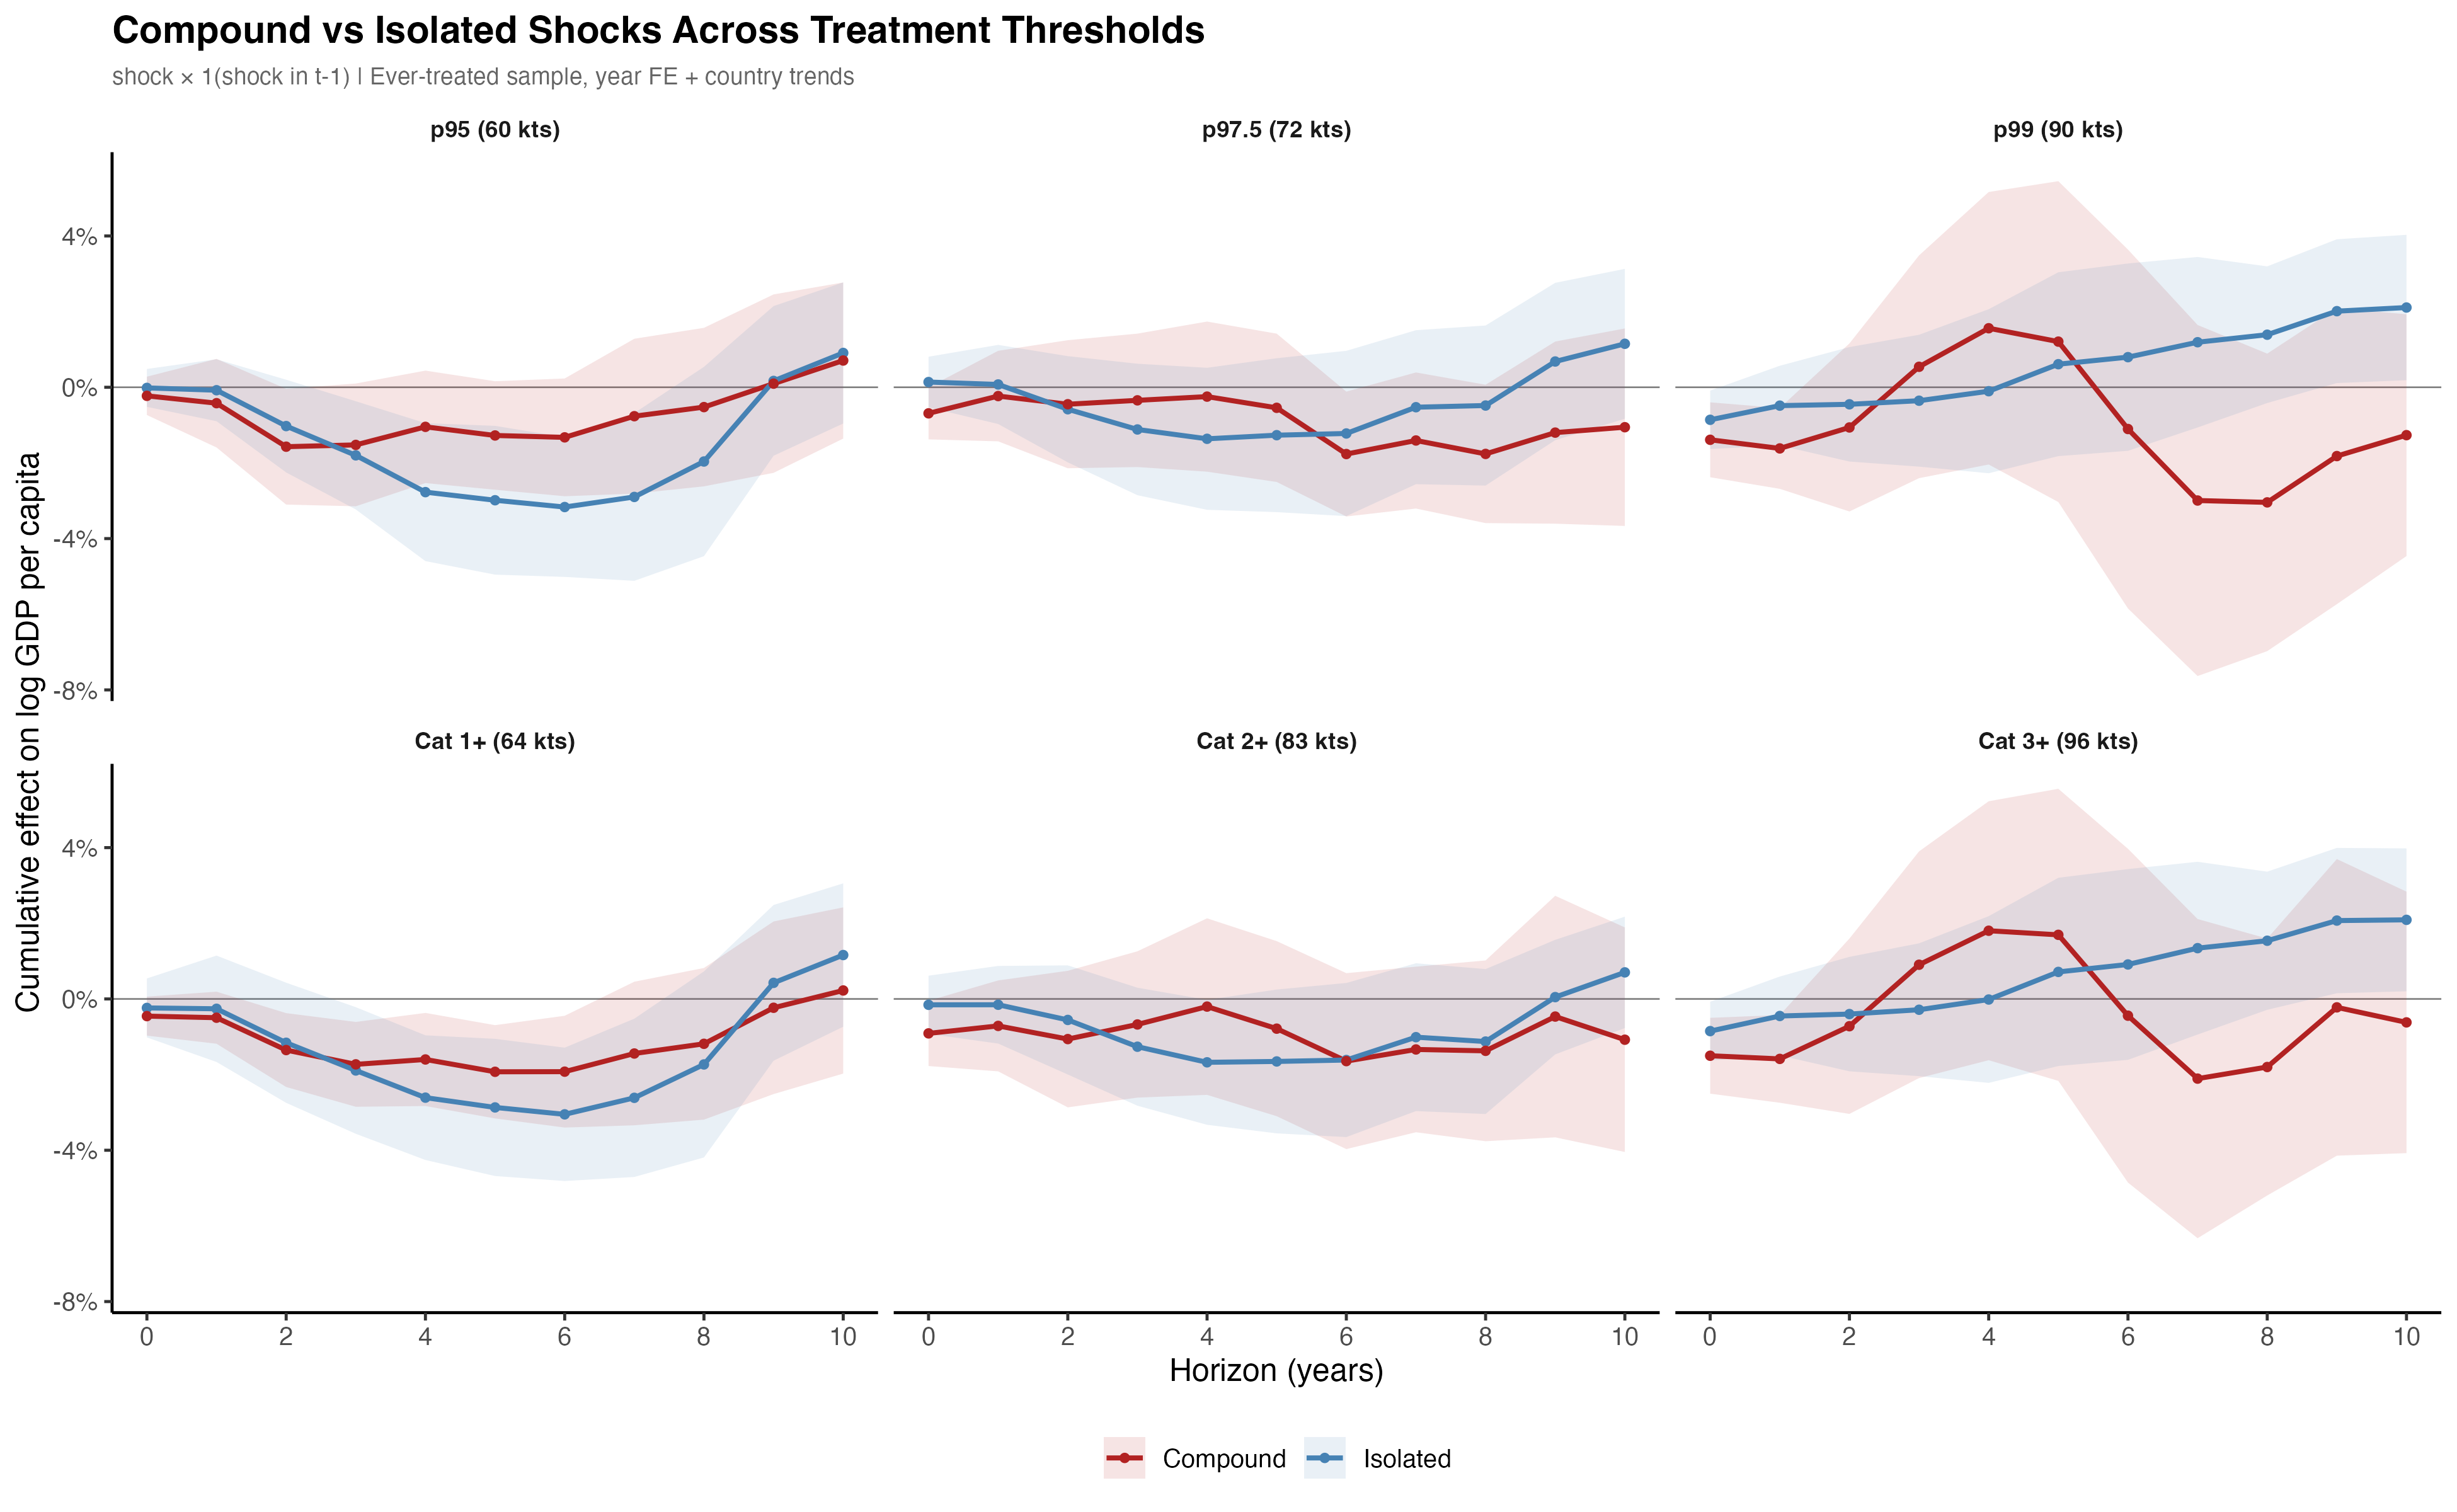
\includegraphics[width=\textwidth,height=0.65\textheight,keepaspectratio]{figures/irf_compound_thresholds.png}

\smallskip
\small
As the threshold increases: (1) effects weaken and lose significance due to smaller samples; (2) at p99 and Cat 3+ ($\sim$100 shocks), both compound and isolated effects are near zero or positive. The compound/isolated gap is most visible at p95 and Cat 1+, where sample sizes are largest.
\end{frame}

\begin{frame}{Compound$-$Isolated Gap Across Thresholds}
\centering
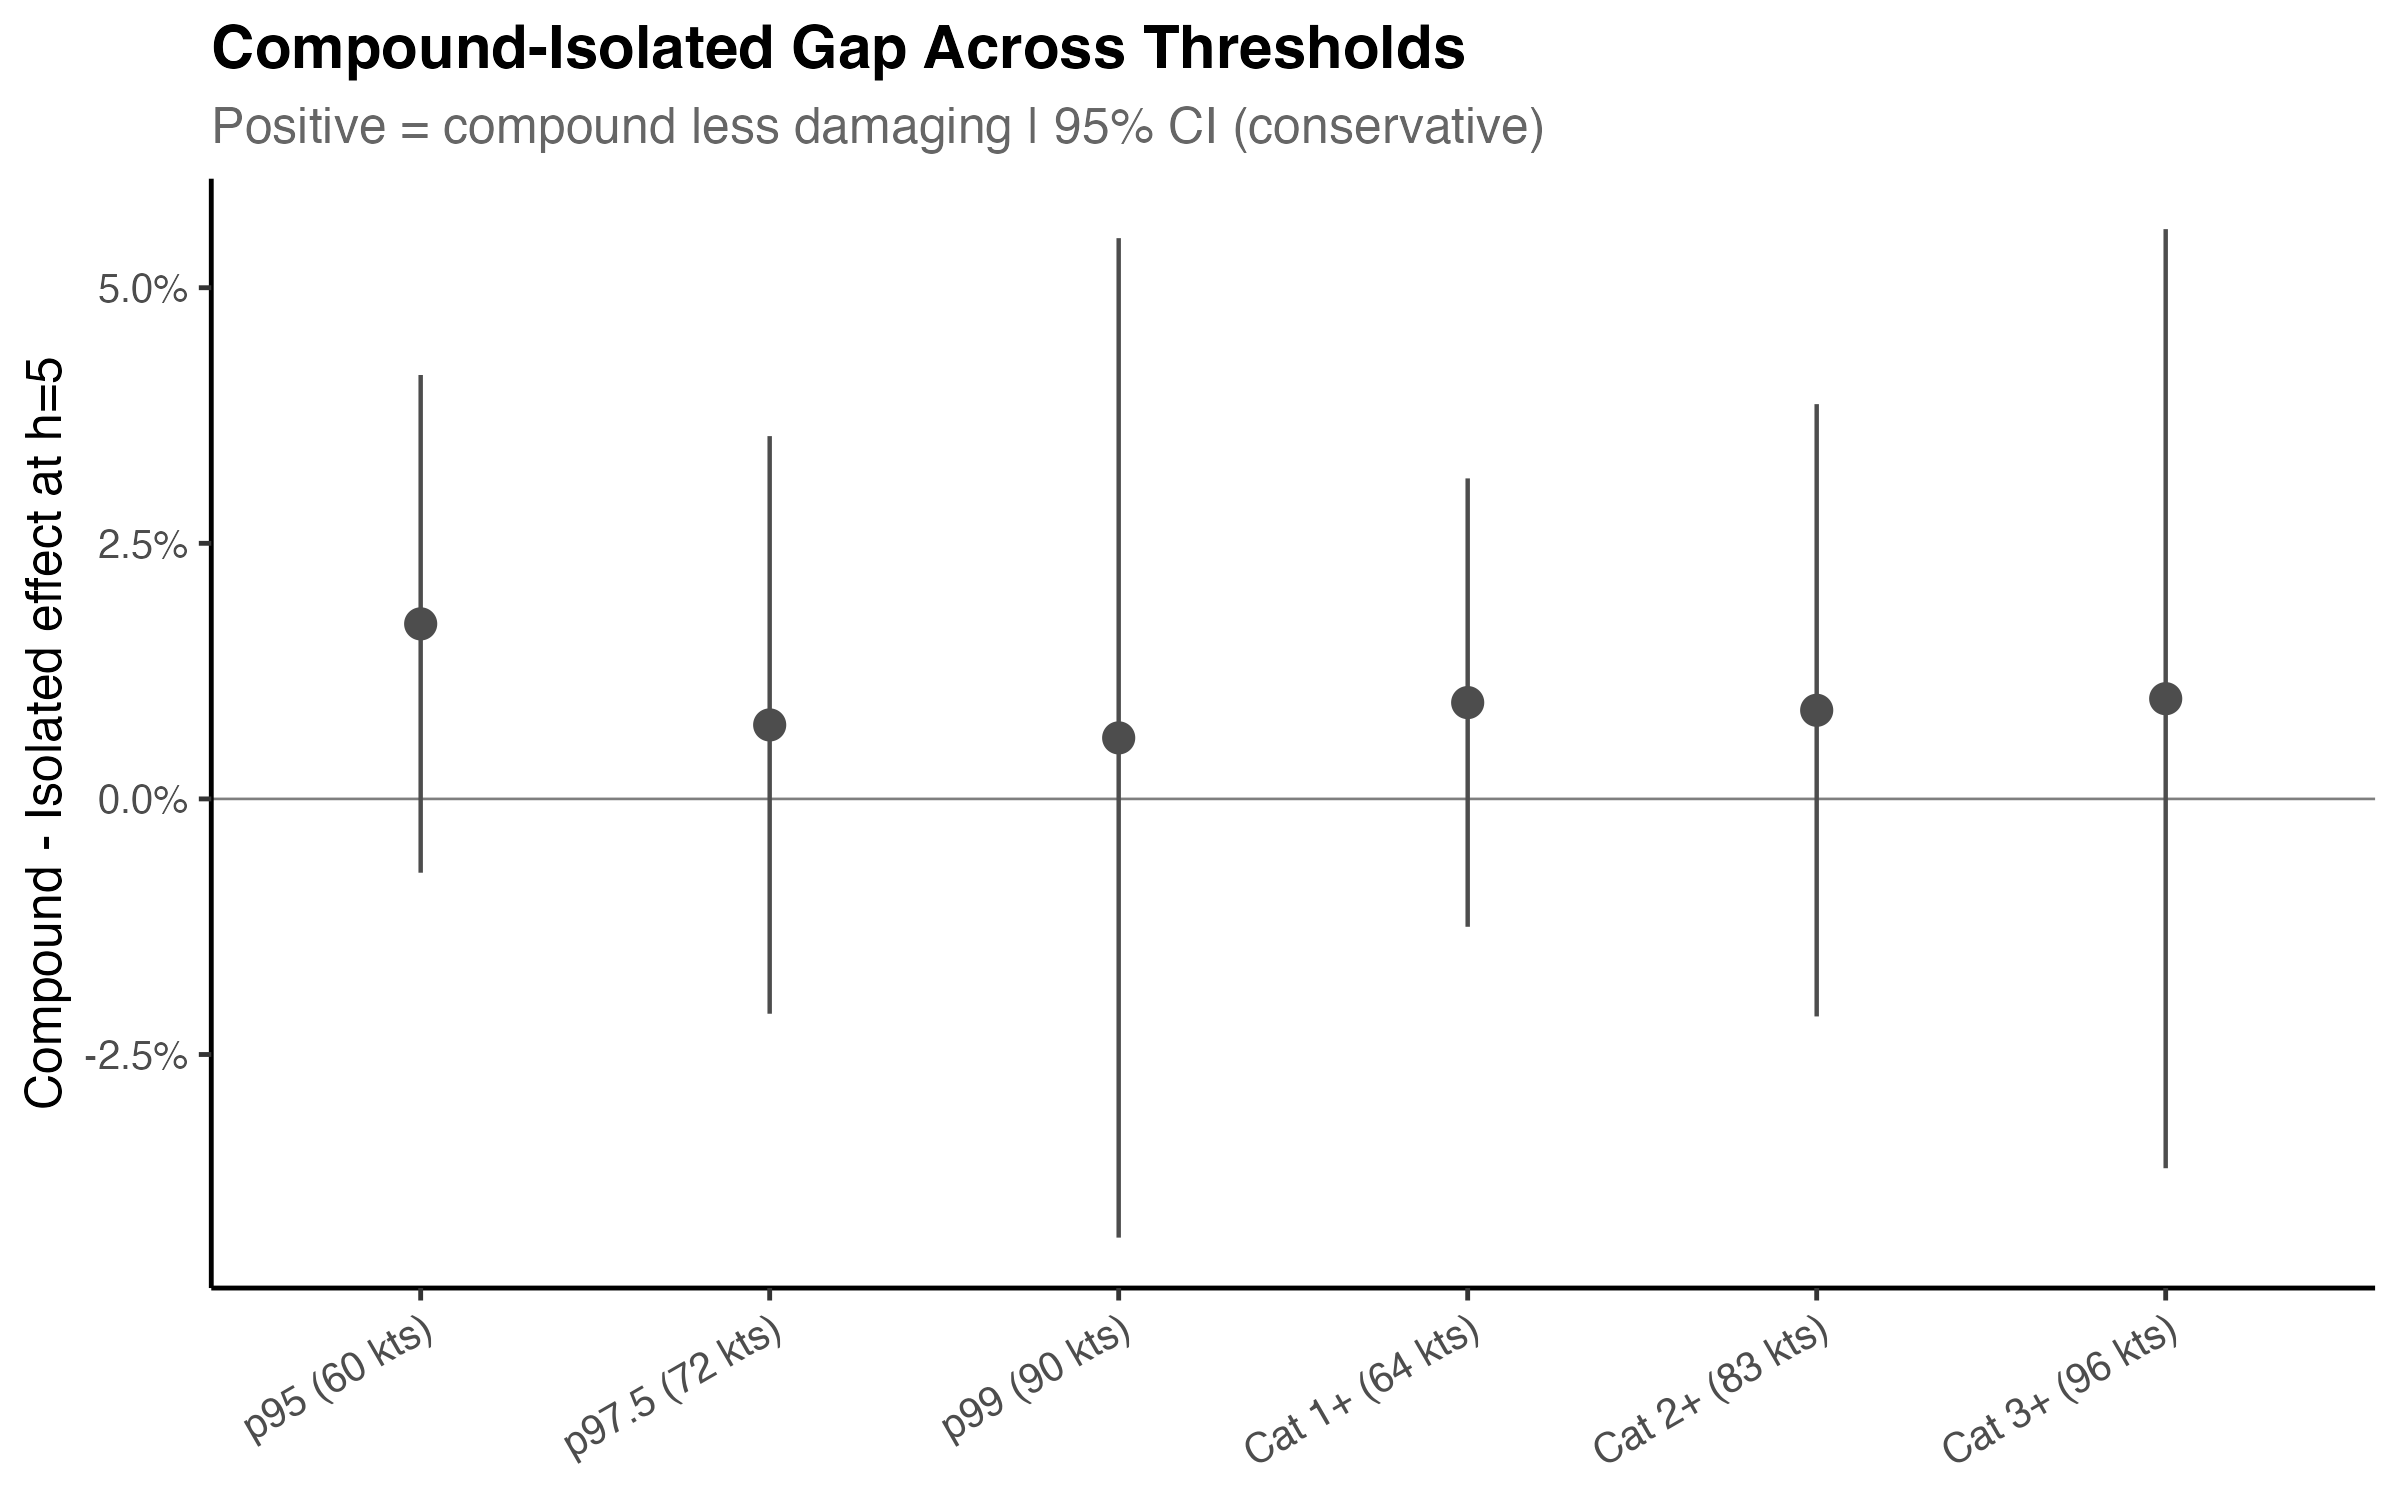
\includegraphics[width=0.72\textwidth,height=0.58\textheight,keepaspectratio]{figures/threshold_gap.png}

\smallskip
\small
The gap (compound $-$ isolated) at $h = 5$ is \textbf{positive} at every threshold --- compound shocks are consistently less damaging. But the gap is \textbf{never significant} and is largest at the lowest threshold where compound-heavy countries dominate.
\end{frame}

\begin{frame}{Threshold Summary}
\centering
\begin{tabular}{l r r r r r}
\hline
\textbf{Threshold} & \textbf{Shocks} & \textbf{Treated} & \textbf{\%Comp} & \textbf{Isol.\ $h{=}5$} & \textbf{Comp.\ $h{=}5$} \\
\hline
p95 (60 kts)   & 423 & 40 & 61.5\% & $-3.0\%$ & $-1.3\%$ \\
p97.5 (72 kts) & 235 & 29 & 47.2\% & $-1.3\%$ & $-0.5\%$ \\
Cat 1+ (64 kts) & 374 & 36 & 58.0\% & $-2.9\%$ & $-1.9\%$ \\
Cat 2+ (83 kts) & 191 & 28 & 40.3\% & $-1.7\%$ & $-0.8\%$ \\
p99 (90 kts)    & 101 & 23 & 17.8\% & $+0.6\%$ & $+1.2\%$ \\
Cat 3+ (96 kts) & 102 & 23 & 18.6\% & $+0.7\%$ & $+1.7\%$ \\
\hline
\end{tabular}

\bigskip
\begin{itemize}
  \item At moderate thresholds (p95--Cat 2+): negative effects, compound less damaging
  \item At severe thresholds (p99, Cat 3+): effects flip positive --- but with only $\sim$100 shocks, power is very limited and CIs are wide
  \item The compound/isolated pattern is qualitatively stable but never statistically significant
\end{itemize}
\end{frame}

% ===============================================================
\section{Interpretation}
% ===============================================================

{\hideframenumber
\begin{frame}
\sectionpage
\end{frame}
\showframenumber}

\begin{frame}{Why Might Compound Shocks Be Less Damaging?}
Several mechanisms could explain the pattern:
\begin{enumerate}
  \item \textbf{Diminishing marginal destruction}: The first shock destroys the most vulnerable capital stock. A second shock has less to destroy --- the remaining infrastructure was either rebuilt to a higher standard or was resilient enough to survive the first shock.

  \medskip
  \item \textbf{Preparedness and learning}: After a shock, governments and households invest in preparedness (early warning, evacuation plans, building codes). A follow-up shock arrives into a better-prepared environment.

  \medskip
  \item \textbf{Mechanical baseline effect}: The LP measures $y_{i,t+h} - y_{i,t-1}$. For compound shocks, $y_{i,t-1}$ is already depressed by the prior shock, so the measured decline from the (lower) baseline is mechanically smaller.

  \medskip
  \item \textbf{Selection on intensity}: Countries that are hit every year (e.g., CHN, PHL) may experience weaker individual storms on average, while isolated shocks may be rarer but more extreme events.
\end{enumerate}
\end{frame}

\begin{frame}{Disentangling the Mechanisms}
\begin{itemize}
  \item The \textbf{continuous intensity} robustness check (Slide~12) is key: when we control for wind speed continuously, the compound/isolated gap disappears. This suggests the binary result reflects \textbf{intensity selection}, not a true interaction effect.

  \medskip
  \item The \textbf{mechanical baseline} concern is partially addressed by the LP design --- $y_{i,t-1}$ is already below trend for compound shocks, so we are measuring the additional damage from this lower starting point. The country trends absorb the systematic component.

  \medskip
  \item The \textbf{diminishing marginal} and \textbf{preparedness} stories are hard to separate without structural modeling, but both predict the observed pattern.
\end{itemize}
\end{frame}

\begin{frame}{Summary and Takeaways}
\begin{enumerate}
  \item \textbf{Isolated shocks appear more damaging} than compound shocks ($-3.0\%$ vs $-1.3\%$ at $h = 5$ with p95), but the difference is \textbf{never statistically significant}.

  \medskip
  \item The pattern is qualitatively \textbf{stable across thresholds} (p95 through Cat 2+), FE specifications, and sample restrictions. At very high thresholds (Cat 3+), effects weaken due to power.

  \medskip
  \item With \textbf{continuous intensity}, the gap disappears --- intensity selection (frequently-hit countries experience weaker storms on average) likely drives much of the binary result.

  \medskip
  \item \textbf{The threshold matters}: The baseline p95 (60 knots) is very low, making countries like AUS and CHN ``treated'' nearly every year. Higher thresholds produce more within-country variation but fewer observations. Cat 2+ (83 knots) offers a reasonable trade-off.

  \medskip
  \item \textbf{No evidence of compounding damage}: Repeated shocks do not amplify GDP losses. Statistical power is limited --- only 19 countries have both types at p95 (fewer at higher thresholds).
\end{enumerate}
\end{frame}

\end{document}
